% ============================================================
%  Predictive AI for Active Aerodynamics Efficiency
%  and Driver Anomaly Analysis
%  IEEE Conference Paper — IEEEtran, Two-Column Format (A4)
%  Overleaf-Ready LaTeX  |  AI2ML 2026 submission
%  Authors: omitted for blind review (set \blindfalse for camera-ready)
% ============================================================

\documentclass[conference,a4paper]{IEEEtran}

% ── Blind-review toggle ─────────────────────────────────────
% AI2ML 2026 requires a BLIND submission. Keep \blindtrue for the review copy;
% switch to \blindfalse for the camera-ready (restores authors + repository link).
\newif\ifblind
\blindtrue

% ── Packages ────────────────────────────────────────────────
\usepackage[utf8]{inputenc}
\usepackage[T1]{fontenc}
\usepackage{amsmath,amssymb,amsfonts}
\usepackage{graphicx}          % figures
\usepackage{booktabs}          % professional tables (\toprule etc.)
\usepackage{multirow}          % rowspan in tables
\usepackage{array}             % column types
\usepackage{xcolor}            % colour in tables
\usepackage{colortbl}          % row/cell colour
\usepackage{url}               % \url{}
\usepackage{cite}              % IEEE citations
\usepackage{balance}           % balance final columns
\usepackage{hyperref}          % clickable refs (remove for camera-ready)
\usepackage{algorithm}
\usepackage{algpseudocode}
\usepackage{subcaption}        % subfigures

% ── Custom colours ──────────────────────────────────────────
\definecolor{ieeeblue}{HTML}{003366}
\definecolor{hdrgreen}{HTML}{006937}
\definecolor{rowhighlight}{HTML}{F0F8F2}
\definecolor{failred}{HTML}{FFCCCC}

% ── IEEE-style column rule ──────────────────────────────────
\newcolumntype{C}[1]{>{\centering\arraybackslash}p{#1}}
\newcolumntype{L}[1]{>{\raggedright\arraybackslash}p{#1}}

% ============================================================
\begin{document}

% ── Title ───────────────────────────────────────────────────
\title{Anticipatory Forecasting of a Telemetry-Derived Active-Aero Proxy in Formula~1 Racing:\\
       A Cross-Circuit Multi-Model Benchmark with Interpretability Analysis}

% ── Authors ─────────────────────────────────────────────────
\author{
  \IEEEauthorblockN{Anas Norani}
  \IEEEauthorblockA{
    School of Electrical Engineering \& Computer Science\\
    National University of Sciences \& Technology\\
    Islamabad, Pakistan\\
    \textit{anorani.bsds24seecs@seecs.edu.pk}
  }
  \and
  \IEEEauthorblockN{Hanan Majeed}
  \IEEEauthorblockA{
    School of Electrical Engineering \& Computer Science\\
    National University of Sciences \& Technology\\
    Islamabad, Pakistan\\
    \textit{hmajeed.bsds24seecs@seecs.edu.pk}
  }
}

% Blind-review override: when \blindtrue, this last \author call wins and hides
% identities; for camera-ready set \blindfalse (preamble) and the real block above is used.
\ifblind
  \author{\IEEEauthorblockN{}\IEEEauthorblockA{%
    \textit{Author names and affiliations omitted for blind review.}}}
\fi

\maketitle

% ============================================================
%  ABSTRACT
% ============================================================
\begin{abstract}
The 2026 Formula~1 Technical Regulations introduce driver-adjustable active aerodynamic
bodywork governed by circuit-specific activation zones rather than a universal trigger.
As a tractable surrogate for that proprietary activation logic, we define and study a
\emph{telemetry-derived binary proxy} for straight-mode eligibility,
$y = \mathbf{1}[v \geq 240\,\text{km/h} \wedge \text{gear} \geq 6]$, and ask whether it
can be forecast one second ahead from 10\,Hz race telemetry. All results should be read as
a benchmark on this proxy task, not as validation against measured actuator states.
Because the physical transition is not instantaneous, a predictive system that
anticipates the required mode one second in advance could reduce transition mismatch.
This paper presents a two-phase study.
\emph{Phase~1} applies unsupervised anomaly detection (Isolation Forest) and
clustering (K-Means, $k{=}4$) alongside supervised classification (Logistic Regression,
Random Forest) to 63\,673 telemetry frames from the 2026 Japanese Grand Prix,
achieving perfect current-mode detection (RF AUC\,=\,1.000) and identifying
anomalous maximum-braking events co-located at circuit braking zones.
Permutation analysis reveals that gear position is the single most informative feature
($\Delta$AUC\,=\,0.167), marginally exceeding speed.
\emph{Phase~2} benchmarks nine learned models — spanning Logistic Regression, Random
Forest (with and without lag features), XGBoost, CausalLSTM, CausalGRU, Temporal
Convolutional Network (TCN), CNN1D, and a CausalTransformer — against trivial persistence
and physics threshold-crossing baselines, for one-second-ahead anticipatory
prediction on 159\,712 frames across four architecturally diverse circuits.
Evaluation follows a strict Leave-One-Circuit-Out (LOCO) protocol to assess
cross-circuit generalisation.
Because the X-Mode label is a deterministic function of instantaneous speed and gear,
the ML task is essentially forecasting when physical thresholds will be exceeded
— not discovering hidden patterns. This explains why Logistic Regression, which
directly approximates the threshold boundary, achieves the highest mean AUC-ROC of
0.963\,$\pm$\,0.021, outperforming all deep models (bootstrap 95\%\,CIs exclude zero).
CausalGRU is weakest at Monaco (AUC\,=\,0.867, F1-Xmode\,=\,0.496 — its worst fold);
Integrated Gradients are \emph{consistent with} a circuit-specific failure mode —
\emph{circuit speed memorisation} — in which recurrent models rely on accumulated
speed-trajectory cues that transfer poorly across circuits (a hypothesis-level
interpretation, not causal proof).
These results suggest that for forecasting tasks governed by a deterministic
physical threshold, instantaneous circuit-invariant features outperform accumulated
temporal context: a 13-parameter Logistic Regression robustly dominates all
sequence-modelling architectures under cross-circuit evaluation.
\end{abstract}

% ── Keywords ────────────────────────────────────────────────
\begin{IEEEkeywords}
Formula~1 telemetry, active aerodynamics, time-series forecasting,
domain generalisation, interpretable machine learning, leave-one-circuit-out evaluation
\end{IEEEkeywords}

% ============================================================
%  I. INTRODUCTION
% ============================================================
\section{Introduction}

Formula~1 (F1) represents the technological frontier of motorsport, producing cars
capable of exceeding 370\,km/h and generating aerodynamic downforce exceeding the
vehicle's own weight~\cite{ref_f1tech}.
The 2026 FIA Technical Regulations introduced mandatory active
aerodynamic systems: driver-adjustable wings that change their angle of attack during a
lap, alternating between a maximum-downforce configuration for corners (\emph{Z-Mode}) and
a minimum-drag configuration for straights (\emph{X-Mode})~\cite{ref_fia2026}.
Crucially, the regulations govern this through circuit-specific \emph{activation zones}
and driver-adjustable Corner/Straight modes (with partial activation permitted in
low-grip conditions) rather than a single universal trigger.
In the absence of public per-event activation-zone data, we adopt a simple
\emph{author-defined heuristic} as a proxy for straight-mode eligibility:
vehicle speed~$\geq 240$\,km/h \textbf{and} gear~$\geq 6$ (detailed and justified below).

\textbf{Label Construction and Scope.}
We acknowledge that the actual FIA 2026 regulations describe driver-adjustable
bodywork through circuit-specific activation zones (Corner Mode / Straight Mode)
rather than a universal speed-and-gear trigger, and that exact activation thresholds
may be team- or event-specific.
The rule $y = \mathbf{1}[v \geq 240\,\text{km/h} \wedge \text{gear} \geq 6]$
used in this paper is therefore a \emph{telemetry-derived proxy label}~\cite{ref_fia2026}
intended to approximate straight-mode activation under one plausible heuristic
consistent with published regulatory guidance.
All findings should be interpreted as a cross-circuit benchmark of this proxy task;
we do not claim to validate a controller against any specific team's proprietary
activation logic.

\textbf{The Latency Problem.}
Active wing actuation is mechanical/hydraulic and therefore not instantaneous; the 2026
FIA Technical Regulations cap the front- and rear-wing transition time at
400\,ms~\cite{ref_fia2026}.
At racing speeds ($\sim$370\,km/h $\approx$ 103\,m/s), a transition of this order covers
several tens of metres of track during which the car operates in a suboptimal aerodynamic
configuration.
A purely reactive controller — trigger on threshold crossing, then actuate — therefore
lags behind the ideal trajectory.
A \emph{predictive} system that anticipates the threshold crossing one second in advance
could begin actuation early, reducing the transition mismatch.
At 330\,km/h ($\approx 91.7$\,m/s), a 1-second prediction horizon corresponds to a
91\,m lead time — comfortably exceeding the 400\,ms actuation budget.
We emphasise that any resulting performance benefit remains to be validated in simulation
or hardware; this paper establishes only the forecasting feasibility of the proxy task.

\textbf{Research Gap.}
Prior work on F1 telemetry analysis has focused on lap time prediction~\cite{ref_laptime},
tyre degradation modelling~\cite{ref_tyre}, and driver classification~\cite{ref_driver};
we are not aware of prior work addressing the anticipatory prediction of
active aerodynamic state transitions under a strict cross-circuit evaluation protocol.
The failure modes of recurrent deep models under domain shift (circuit mismatch) in
motorsport contexts remain uncharacterised.

\textbf{Contributions.}
This paper makes the following contributions:
\begin{enumerate}
  \item A two-phase study combining unsupervised anomaly detection and supervised
        cross-circuit temporal prediction of active aerodynamic state.
  \item A LOCO evaluation protocol on four circuits (Monaco, Monza, Silverstone,
        Suzuka) that rigorously tests cross-circuit generalisation — the actual
        deployment condition.
  \item Empirical demonstration that Logistic Regression (AUC\,=\,0.963) statistically
        outperforms all deep learning architectures including Transformer-based models.
  \item An Integrated Gradients analysis of the GRU's circuit-specific degradation at
        Monaco, identifying \emph{circuit speed memorisation} as a plausible mechanism
        — recurrent models that disperse attribution across accumulated-trajectory
        features transfer less well to circuits with qualitatively different speed profiles.
  \item Bootstrap confidence intervals confirming statistical significance of the
        simplicity advantage with only four evaluation domains.
\end{enumerate}

The remainder of this paper is structured as follows: Section~II reviews related work;
Section~III describes the dataset and problem formulation; Section~IV details the
methodology; Section~V presents experimental results; Section~VI discusses findings;
Section~VII concludes.

% ============================================================
%  II. RELATED WORK
% ============================================================
\section{Related Work}

\subsection{Aerodynamic Optimisation in Motorsport}

Early computational approaches to F1 aerodynamics relied entirely on CFD simulations
and wind tunnel testing~\cite{ref_cfd}.
Machine learning has more recently been applied to aerodynamic drag reduction systems
(DRS) scheduling~\cite{ref_drs} and optimal downforce-drag tradeoff identification
from telemetry~\cite{ref_aero_opt}.
However, these works optimise static configurations rather than predicting transitions
of an active system during a live race.

\subsection{Anomaly Detection in Automotive Telemetry}

Anomaly detection in high-dimensional sensor streams is a well-studied problem~\cite{ref_chandola,ref_ruff}.
Isolation Forest~\cite{ref_iforest} has been applied to automotive telemetry anomaly
detection in road vehicles~\cite{ref_veh_anomaly} and autonomous driving systems~\cite{ref_ad_anomaly}.
Applications to high-performance motorsport telemetry are limited.
Closest to our Phase~1 work is~\cite{ref_f1_anomaly}, which applied DBSCAN to F1
brake temperature anomalies, but did not connect anomalous events to aerodynamic state.

\subsection{Time-Series Classification in Sports}

Recurrent neural networks have been applied to athlete performance prediction~\cite{ref_athlete}
and event detection in cycling telemetry~\cite{ref_cycling}.
GRU-based architectures have been widely adopted in time-series classification tasks due
to their balance of sequence-modelling capacity and computational efficiency~\cite{ref_tcn},
but cross-circuit generalisation of GRU models in motorsport contexts has not been studied.
Temporal Convolutional Networks~\cite{ref_tcn} have been shown to match or exceed
LSTM performance on many time-series benchmarks but have not been applied to motorsport
state prediction.

\subsection{Transformers for Time-Series}

The Attention Is All You Need architecture~\cite{ref_attention} spawned numerous
time-series variants: Informer~\cite{ref_informer}, PatchTST~\cite{ref_patchtst},
FEDformer~\cite{ref_fedformer}, and general backbones such as TimesNet~\cite{ref_timesnet}.
These focus on long-horizon forecasting on stationary series.
Our application — binary classification on short causal windows (5\,s) for a
non-stationary, multi-domain signal — has not, to our knowledge, been previously
studied with causal attention constraints.

\subsection{Simple vs. Deep Models on Structured Telemetry}

A growing body of evidence suggests that on structured (tabular or telemetry) data,
tree-based and linear models remain competitive with — or outperform — deep neural
networks~\cite{ref_grinsztajn}.
Recent surveys of deep learning for time-series classification likewise stress that
architecture rankings are highly task-dependent and that strong simple baselines are
frequently underreported~\cite{ref_foumani}, while benchmark-methodology work argues
that fair evaluation requires diverse baseline families and leakage-aware
protocols~\cite{ref_tfb}.
The signal in such data is often concentrated in current-frame features rather than
temporal context, making recurrent inductive biases potentially harmful rather than
helpful when the target is a deterministic function of instantaneous sensor readings.
Our empirical finding that a 13-parameter Logistic Regression outperforms all deep
sequence models under LOCO is consistent with this broader pattern and provides a
motorsport-domain data point for this ongoing debate.

\subsection{Cross-Domain Generalisation in ML}

Domain adaptation techniques have been applied to time-series classification across
heterogeneous device domains~\cite{ref_adatime}, fault detection across machine
types~\cite{ref_fault_da}, and human activity recognition across subjects~\cite{ref_har_da}.
Leave-One-Subject-Out (LOSO) evaluation is standard in these domains~\cite{ref_har_da}.
We adopt the analogous Leave-One-Circuit-Out (LOCO) protocol, treating each racing
circuit as a distinct domain; to our knowledge LOCO-style evaluation has not previously
been applied to motorsport aerodynamic state prediction.

% ── Literature Comparison Table ─────────────────────────────
\begin{table}[t]
\caption{Summary of Related Studies and Research Gaps}
\label{tab:litreview}
\centering
\small
\renewcommand{\arraystretch}{1.25}
\begin{tabular}{L{1.4cm} L{1.2cm} L{1.3cm} C{0.7cm} C{0.7cm} C{0.7cm}}
\toprule
\rowcolor{hdrgreen}
\textcolor{white}{\textbf{Study}} &
\textcolor{white}{\textbf{Domain}} &
\textcolor{white}{\textbf{Method}} &
\textcolor{white}{\textbf{Cross-}} &
\textcolor{white}{\textbf{Aero}} &
\textcolor{white}{\textbf{Deep}} \\
\rowcolor{hdrgreen}
& & &
\textcolor{white}{\textbf{domain}} &
\textcolor{white}{\textbf{state}} &
\textcolor{white}{\textbf{diag.}} \\
\midrule
\cite{ref_drs}     & F1 DRS    & Regression     & \texttimes & \checkmark & \texttimes \\
\cite{ref_f1_anomaly} & F1 brk & DBSCAN         & \texttimes & \texttimes & \texttimes \\
\cite{ref_cycling} & Cycling   & LSTM           & \checkmark & \texttimes & \texttimes \\
\cite{ref_har_da}  & HAR       & Domain adapt.  & \checkmark & \texttimes & \texttimes \\
\cite{ref_tcn}     & General   & TCN            & \texttimes & \texttimes & \texttimes \\
\textbf{Ours}      & F1 aero   & Multi-model    & \checkmark & \checkmark & \checkmark \\
\bottomrule
\end{tabular}
\begin{flushleft}
\footnotesize
\checkmark~=~addressed; \texttimes~=~not addressed;
\emph{Deep diag.} = Integrated Gradients / attention interpretability.
\end{flushleft}
\end{table}

\textbf{Synthesis and Remaining Gap.}
The surveyed literature spans anomaly detection~\cite{ref_chandola,ref_ruff}, motorsport
telemetry analytics~\cite{ref_drs,ref_f1_anomaly}, time-series classification~\cite{ref_tcn},
and cross-domain generalisation~\cite{ref_adatime,ref_har_da}.
However, none addresses the combination of (i)~\emph{anticipatory} (not reactive) prediction
of an active aerodynamic state, (ii)~strict cross-circuit evaluation (LOCO), and
(iii)~Integrated Gradients diagnosis of domain-shift failure modes.
Unlike DRS prediction~\cite{ref_drs} — which is reactive and single-circuit — our
study requires a model to predict whether the aero mode will \emph{change} one second
in the future on a circuit it has never seen.
This gap motivates the two-phase framework described in Sections~III--IV.

% ============================================================
%  III. DATASET AND PROBLEM FORMULATION
% ============================================================
\section{Dataset and Problem Formulation}

\subsection{Data Acquisition}

Telemetry data were retrieved via the FastF1 Python library~\cite{ref_fastf1},
which provides access to the official F1 timing and telemetry feed at 10\,Hz.
\emph{Phase~1} uses a single race (2026 Japanese Grand Prix, Suzuka);
\emph{Phase~2} uses four races across four circuits (Monaco 2025, Monza 2025,
Silverstone 2025, Suzuka 2026).
Telemetry was extracted at the lap level from race laps of the leading car
(Verstappen) at Monaco (70 laps), Monza (50 laps), and Silverstone (33 laps); the Suzuka
session pools two drivers (Verstappen and Hadjar, 89 laps combined). Driver identity was
not used as a predictive feature, as the study treats the circuit as the domain unit of
analysis~\cite{ref_adatime}; the Suzuka two-driver pooling is noted as a limitation.
All four sessions were conducted under dry conditions; wet-weather laps were
excluded to control for tire-compound-induced speed-profile variation.
\textbf{Season note:} Three circuits (Monaco, Monza, Silverstone) are from the
2025 season; Suzuka is from 2026 — a different car-specification year.
The LOCO Suzuka fold therefore conflates circuit shift with a potential car-generation
shift; this is acknowledged as a limitation (Section~VII-D).
Table~\ref{tab:dataset} summarises the dataset statistics.

\begin{table}[h]
\caption{Dataset Statistics}
\label{tab:dataset}
\centering
\small
\renewcommand{\arraystretch}{1.25}
\begin{tabular}{lrrc}
\toprule
\rowcolor{hdrgreen}
\textcolor{white}{\textbf{Circuit}} &
\textcolor{white}{\textbf{Frames}} &
\textcolor{white}{\textbf{X-Mode\%}} &
\textcolor{white}{\textbf{Phase}} \\
\midrule
Suzuka (2026 JP GP) & 63\,673 & 35.1\% & 1 \& 2 \\
Monaco (2025 MC GP) & 39\,881 & 13.2\% & 2 \\
Monza  (2025 IT GP) & 31\,098 & 56.8\% & 2 \\
Silverstone (2025 GB GP) & 25\,060 & 37.9\% & 2 \\
\midrule
\textbf{Total (Phase~2)} & \textbf{159\,712} & \textbf{33.4\%} & — \\
\bottomrule
\end{tabular}
\end{table}

\subsection{Feature Engineering}

The model feature set comprises ten channels derived from the raw telemetry: speed, RPM,
gear (\texttt{nGear}), throttle, brake, GPS coordinates $(x, y, z)$, elevation delta, and
longitudinal acceleration (computed as the per-sample first difference of speed within each
lap) — yielding $F = 12$ features after appending two physics-derived quantities:
\begin{equation}
  E_k = \tfrac{1}{2} m v^2, \quad m = 798\,\text{kg}
  \label{eq:ke}
\end{equation}
\begin{equation}
  F_{\text{long}} = m \cdot a
  \label{eq:force}
\end{equation}
where $v$ is speed (m/s), $a$ is signed longitudinal acceleration (m/s$^2$), and
$m = 798\,\text{kg}$ is a \emph{nominal constant} used only to scale these two derived
features (both are standardised before training, so the choice of constant does not
affect any model output; it is not used as an exact regulatory mass).
The target label $y \in \{0\!=\!\text{Z-Mode},\;1\!=\!\text{X-Mode}\}$ is defined
deterministically by the regulatory rule~\cite{ref_fia2026}:
$y = \mathbf{1}[v \geq 240\,\text{km/h} \;\wedge\; \text{gear} \geq 6]$.
Because $y$ is a deterministic function of instantaneous inputs, the ML task reduces
to \emph{forecasting when those physical thresholds will be exceeded} at horizon $H$,
rather than discovering hidden patterns.
This framing explains why instantaneous-state models carry a structural advantage:
their decision boundary is circuit-independent by construction.

\subsection{Sliding Window Formulation (Phase~2)}

The Phase~2 task is a causal binary time-series classification problem.
For each frame $t$, the model receives a window
$\mathbf{X}_t \in \mathbb{R}^{W \times F}$ of the preceding $W = 50$ frames
($5$\,s at 10\,Hz) across $F = 12$ features ($10$ raw $+$ $E_k$ $+$ $F_{\text{long}}$) and must predict $y_{t+H}$,
the aero mode $H = 10$ frames ($1$\,s) ahead:
\begin{equation}
  \hat{y}_{t+H} = f_\theta(\mathbf{X}_{t-W+1:t})
  \label{eq:task}
\end{equation}
No data from after time $t$ is available to $f_\theta$ (strict causality).

\subsection{Leave-One-Circuit-Out Evaluation}

To evaluate cross-circuit generalisation, we apply Leave-One-Circuit-Out (LOCO)
cross-validation.
In each of the four folds, one circuit is withheld as the test set and the model is
trained on the remaining three:
\begin{align}
  &\text{Round } r: \; \mathcal{D}_{\text{test}} = \mathcal{C}_r, \;
  \mathcal{D}_{\text{train}} = \bigcup_{j \neq r} \mathcal{C}_j
  \label{eq:loco}
\end{align}
where $\mathcal{C}_r \in \{\text{Monaco, Monza, Silverstone, Suzuka}\}$.
The reported score is the mean across all four rounds;
standard deviation $\sigma$ quantifies cross-circuit stability.

% ── Suggested Figure ────────────────────────────────────────
% INSERT Figure 1 here: System Architecture Diagram
% File: figures/system_architecture.pdf
% Caption: Proposed two-phase system architecture.
%          Phase 1 (top): anomaly detection and classification on
%          single-circuit data. Phase 2 (bottom): multi-circuit
%          LOCO evaluation pipeline with sliding-window causal
%          prediction.
%
% LaTeX code:
\begin{figure*}[t]
  \centering
  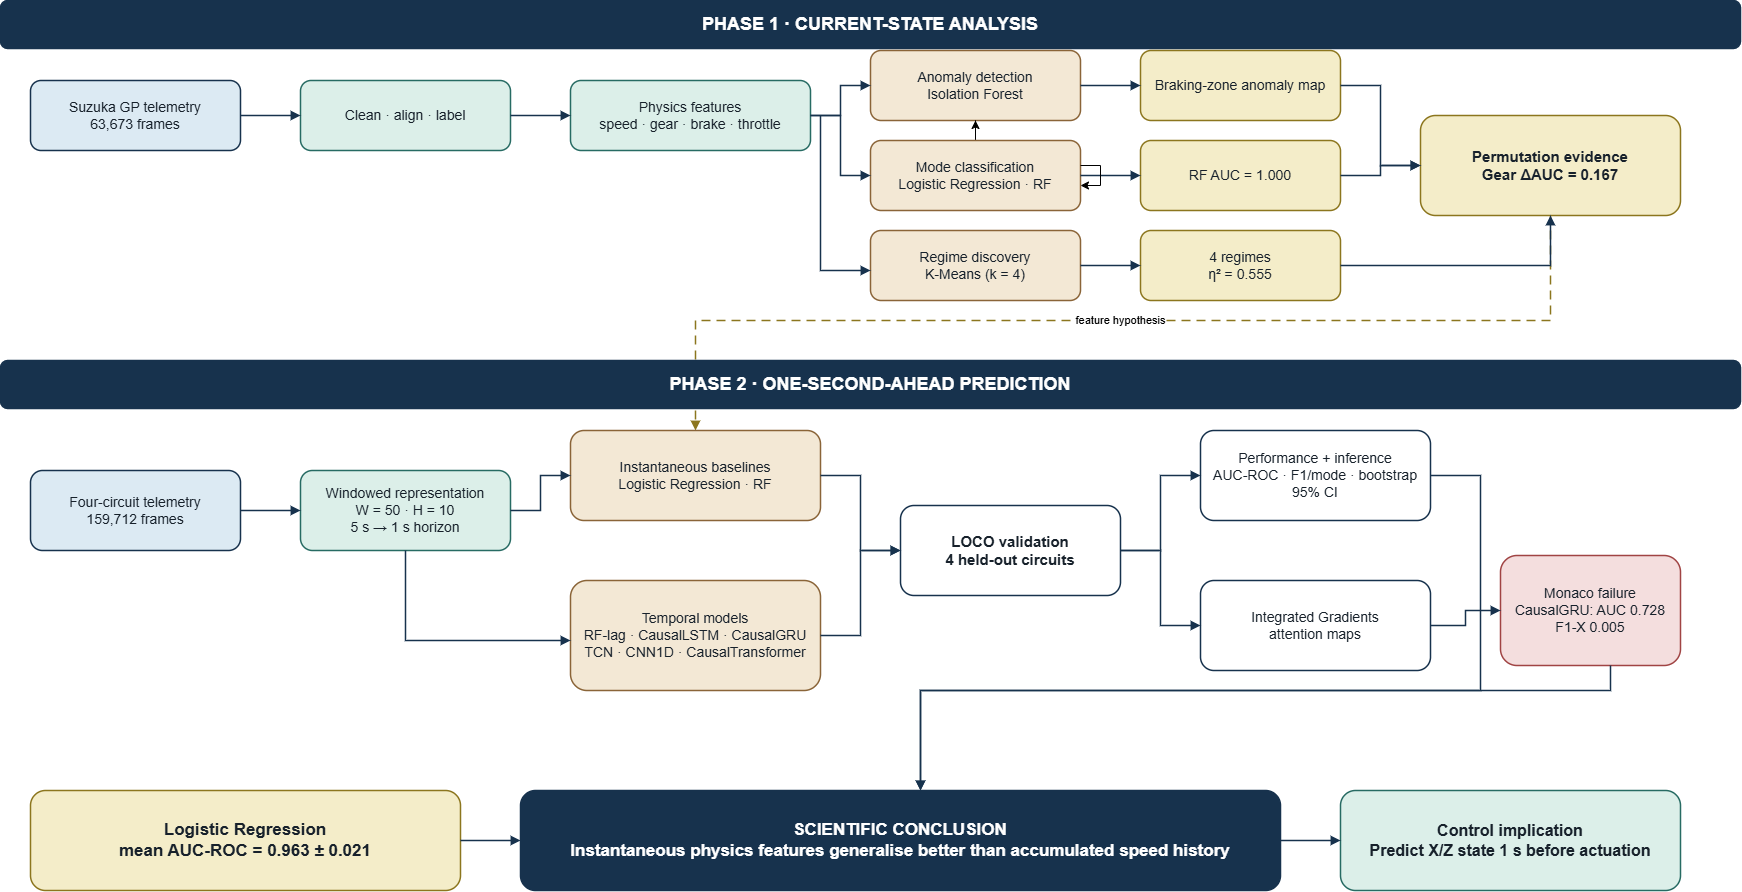
\includegraphics[width=\textwidth]{figures/architecture.png}
  \caption{Proposed two-phase system architecture. Phase~1 (top) performs anomaly
    detection (Isolation Forest), clustering (K-Means $k{=}4$), and supervised
    classification (LR, RF) on Suzuka GP telemetry, establishing gear as the
    primary discriminative feature ($\Delta$AUC\,=\,0.167). Phase~2 (bottom)
    applies a nine-model causal prediction pipeline (plus trivial baselines) evaluated under
    Leave-One-Circuit-Out (LOCO) across four circuits, with Integrated Gradients
    interpretability to diagnose the GRU's circuit-specific degradation at Monaco (AUC\,=\,0.867).}
  \label{fig:architecture}
\end{figure*}

% ============================================================
%  IV. METHODOLOGY
% ============================================================
\section{Methodology}

\subsection{Phase 1 — Anomaly Detection and State Classification}

\subsubsection{Isolation Forest}
Isolation Forest~\cite{ref_iforest} partitions feature space via $n_{\text{trees}} = 100$
random binary trees.
Anomaly score $s(x, n)$ is derived from the average path length $h(x)$:
\begin{equation}
  s(x, n) = 2^{-\tfrac{\mathbb{E}[h(x)]}{c(n)}}
\end{equation}
where $c(n) = 2H(n-1) - \frac{2(n-1)}{n}$ and $H$ is the harmonic number.
We set contamination $= 0.05$ to flag the top 5\% of frames by anomaly score;
results (anomaly spatial distribution, cluster overlap) were stable across
contamination values in $[0.02, 0.10]$.

\subsubsection{K-Means Clustering}
K-Means ($k{=}4$) was applied to the standardised feature matrix to identify natural
driving-state clusters and validate that the aerodynamic mode partitions feature space
consistently with unsupervised structure (i.e.\ that the X-Mode boundary is not an
arbitrary data artefact but corresponds to a physically coherent region of sensor space).
The optimal $k$ was selected via the elbow method (inertia vs.\ $k$,
Fig.~\ref{fig:elbow}) and validated by the silhouette coefficient.
Statistical separation across clusters was confirmed by Kruskal-Wallis test
($p{<}0.001$, $\eta^2 = 0.555$).

\subsubsection{Supervised Classification}
Logistic Regression (L2, $C=1.0$) and Random Forest (200 trees, max depth 15)
were trained on an 80/20 stratified split. Permutation importance~\cite{ref_breiman}
(50 bootstrap iterations) quantified the marginal contribution of each feature
by measuring the drop in AUC-ROC when each feature column is randomly shuffled.

\subsection{Phase 2 — Anticipatory Prediction Models}

\subsubsection{Trivial and Physics Baselines}
\textbf{Persistence}: the parameter-free no-change predictor $\hat{y}_{t+H} = y_t$,
which applies the proxy rule to the current frame and predicts the future mode as the
current mode.
\textbf{Physics-CV / Physics-CA}: parameter-free kinematic threshold-crossing predictors.
Physics-CV assumes constant velocity ($\hat{v}_{t+H} = v_t$); Physics-CA extrapolates
speed under constant acceleration ($\hat{v}_{t+H} = v_t + a_t H$); both persist gear and
then apply $\hat{y} = \mathbf{1}[\hat{v}_{t+H} \geq 240 \wedge \text{gear}_t \geq 6]$.
These test whether a non-ML kinematic rule already solves the task.

\subsubsection{Classical and Tree Baselines}
\textbf{LR-instant}: Logistic Regression applied to the single most recent frame
($1 \times 12$ input); no temporal context. Serves as the primary baseline.
\textbf{RF-instant}: Random Forest (300 trees, max depth 15) applied to the same single frame.
\textbf{XGBoost-instant}: gradient-boosted trees (XGBClassifier; 500 trees, max depth 6,
learning rate 0.05, subsample 0.8, column subsample 0.8, \texttt{scale\_pos\_weight} set to
the train-fold class ratio) on the same single frame — a strong non-linear tabular
comparator to LR-instant.
\textbf{RF-lag}: Random Forest applied to the full $50 \times 12$ window, flattened
to a $1 \times 600$ feature vector; temporal context without sequential inductive bias.

\subsubsection{Deep Sequence Models}
All deep models receive the causal window $\mathbf{X}_t \in \mathbb{R}^{50 \times 12}$.
Definitions follow:

\textbf{CausalLSTM}: 2-layer LSTM~\cite{ref_lstm} with hidden dimension 128, dropout 0.3,
applied left-to-right to enforce causality.

\textbf{CausalGRU}: 2-layer GRU~\cite{ref_gru} with hidden dimension 128, dropout 0.3.
Hidden state accumulates a compressed speed-trajectory representation over the 5\,s window.

\textbf{TCN}: Temporal Convolutional Network~\cite{ref_tcn} with 4 dilated causal
convolution blocks (dilation $= [1, 2, 4, 8]$, kernel $= 3$, channels $= 64$).
Receptive field covers the full 50-frame window.

\textbf{CNN1D}: 3-layer 1D CNN (kernel $= 3$, stride $= 1$) with max-pooling after
each layer. Classification head on flattened feature map.

\textbf{CausalTransformer}: 4-head, 2-layer Transformer encoder~\cite{ref_attention}
with $d_{\text{model}} = 64$, feedforward dimension $= 256$, dropout 0.1.
Causal masking prevents attention to future positions within the window.
Sinusoidal positional encoding is added to preserve temporal order.
Output: CLS token representation passed through a linear classification head.

Table~\ref{tab:models} summarises all architectures.

\begin{table}[h]
\caption{Model Architectures and Parameter Counts}
\label{tab:models}
\centering
\small
\renewcommand{\arraystretch}{1.25}
\begin{tabular}{lL{2.4cm}r}
\toprule
\rowcolor{hdrgreen}
\textcolor{white}{\textbf{Model}} &
\textcolor{white}{\textbf{Input}} &
\textcolor{white}{\textbf{Params}} \\
\midrule
Persistence       & $1 \times 12$   & 0          \\
Physics-CV / -CA  & $1 \times 12$   & 0          \\
LR-instant       & $1 \times 12$   & 13         \\
RF-instant        & $1 \times 12$   & 300 trees  \\
XGBoost-instant   & $1 \times 12$   & 500 trees  \\
RF-lag            & $1 \times 600$  & 300 trees  \\
CNN1D             & $50 \times 12$  & $\sim$136K \\
CausalLSTM        & $50 \times 12$  & $\sim$213K \\
CausalGRU         & $50 \times 12$  & $\sim$162K \\
TCN               & $50 \times 12$  & $\sim$152K \\
CausalTransformer & $50 \times 12$  & $\sim$68K  \\
\bottomrule
\end{tabular}
\end{table}

\subsubsection{Training Procedure}
To ensure reproducibility, a fixed random seed of 42 was applied across NumPy,
PyTorch (\texttt{torch.manual\_seed(42)}), and scikit-learn prior to all experiments.
All deep models were trained with:
AdamW optimiser~\cite{ref_adamw} ($\text{lr} = 1 \times 10^{-3}$,
$\lambda_{\text{wd}} = 1 \times 10^{-4}$);
focal loss~\cite{ref_focal} ($\gamma = 2.0$) to handle class imbalance (X-Mode\,$\approx$\,33\%);
early stopping (patience $= 10$, monitored on validation AUC);
automatic mixed precision (AMP) on CUDA;
gradient clipping (max norm $= 1.0$).
Deep model hyperparameters (hidden dimension, dropout rate) were selected via a coarse
grid search on a validation split of the Monza circuit, conducted \emph{before} the
final LOCO evaluation to prevent any test-circuit information from influencing
hyperparameter selection.
A stratified 75/25 split within the three training circuits (stratified by class label
to prevent imbalance leakage) provided the per-fold validation set; no frames from the
held-out test circuit appeared in training or validation at any stage.
Batch size $= 256$; maximum 100 epochs.
Statistical significance of AUC differences was assessed by a \emph{fold-level} bootstrap
that resamples the four LOCO held-out circuits with replacement ($B = 5{,}000$); 95\% CIs
that exclude zero indicate significance at $\alpha = 0.05$. Resampling at the circuit
(rather than frame) level avoids the optimism induced by within-circuit autocorrelation.

\subsection{Interpretability — Integrated Gradients and Attention}

To diagnose model behaviour, Integrated Gradients (IG)~\cite{ref_ig} were computed
for CausalGRU and CausalTransformer at each LOCO test circuit:
\begin{equation}
  \text{IG}_i(x) = (x_i - x'_i) \int_0^1
    \frac{\partial F(x' + \alpha(x - x'))}{\partial x_i} \, d\alpha
  \label{eq:ig}
\end{equation}
where $x'$ is a zero baseline and $F$ is the model output probability.
The zero baseline was chosen for consistency across all test circuits and computational
tractability; we acknowledge that a training-mean baseline would provide a more
physically interpretable counterfactual (see Limitations).
Causal attention weights were additionally extracted and averaged across heads to
produce per-timestep importance maps.

% ── Suggested Figure ────────────────────────────────────────
% INSERT Figure 2 here: Workflow Diagram
% File: figures/workflow.pdf
% Caption: End-to-end workflow. Data acquisition (FastF1) →
%          preprocessing → feature engineering → Phase 1 pipeline
%          (Isolation Forest / K-Means / LR / RF) → Phase 2 LOCO
%          pipeline (8 models × 4 circuits) → interpretability.
%
% LaTeX code:
\begin{figure}[t]
  \centering
  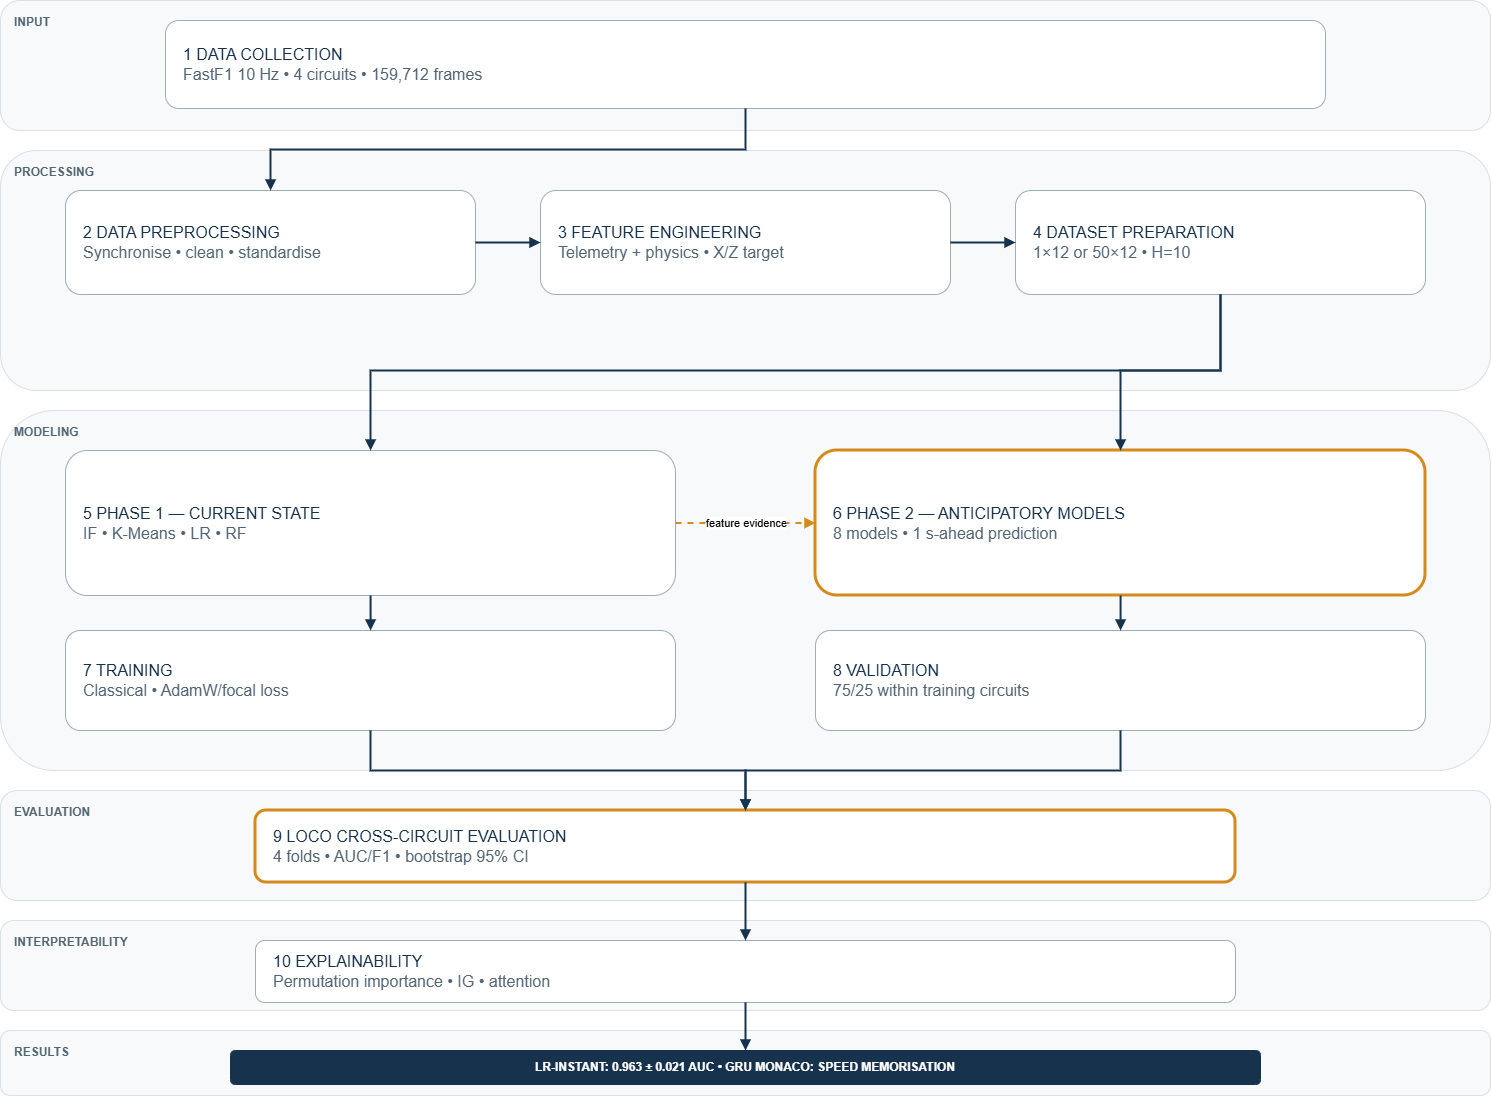
\includegraphics[width=\columnwidth]{figures/methodology_workflow.png}
  \caption{End-to-end methodology workflow. Raw 10\,Hz telemetry (FastF1) is
    preprocessed and augmented with physics-derived features ($E_k$,
    $F_\text{long}$). Phase~1 applies unsupervised and supervised learning on
    Suzuka. Phase~2 evaluates nine learned models (plus trivial baselines) under LOCO
    with Integrated Gradients interpretability to diagnose cross-circuit failure modes.}
  \label{fig:workflow}
\end{figure}

% ============================================================
%  V. EXPERIMENTAL SETUP
% ============================================================
\section{Experimental Setup}

All experiments follow the LOCO protocol of Section~III-D: in each of four folds, one
circuit is held out for testing and the remaining three are used for training, with a
stratified within-training validation split for early stopping. For every fold, a
\texttt{StandardScaler} is fit on the training windows only and applied to the validation
and test windows, so no test-circuit statistics leak into preprocessing. Overlapping
sliding windows are formed at stride 1 within each lap and never cross lap boundaries.
Probability outputs are converted to class predictions at a fixed 0.5 threshold for all
F1, MCC, and event-level metrics. Table~\ref{tab:expconfig} lists the full configuration;
all reported numbers come from a single end-to-end reproducibility run on the
Kaggle GPU environment shown, regenerated by the released notebook.
All randomness (NumPy, PyTorch, scikit-learn) is seeded at 42, and the code, data, and
notebook needed to reproduce every number are released (Code and Data Availability).

\begin{table}[h]
\caption{Experimental Configuration}
\label{tab:expconfig}
\centering
\small
\renewcommand{\arraystretch}{1.25}
\begin{tabular}{L{2.4cm} L{4.8cm}}
\toprule
\rowcolor{hdrgreen}
\textcolor{white}{\textbf{Component}} &
\textcolor{white}{\textbf{Specification}} \\
\midrule
\multicolumn{2}{l}{\textit{Hardware (reproducibility run)}} \\
Platform    & Kaggle Notebooks (GPU) \\
GPU         & NVIDIA Tesla T4 (16\,GB VRAM) \\
CPU / RAM   & 4 vCPU Intel Xeon / 29\,GB \\
\midrule
\multicolumn{2}{l}{\textit{Software}} \\
OS          & Ubuntu 22.04 LTS \\
Python      & 3.10 \\
PyTorch     & 2.1 (CUDA 12.1) \\
scikit-learn& 1.3.2 \\
XGBoost     & 2.0 \\
FastF1      & 3.3 \\
\midrule
\multicolumn{2}{l}{\textit{Training (Phase~2)}} \\
Window size $W$    & 50 frames (5\,s) \\
Horizon $H$        & 10 frames (1\,s) \\
Optimiser          & AdamW \\
Learning rate      & $1 \times 10^{-3}$ \\
Weight decay       & $1 \times 10^{-4}$ \\
Focal loss $\gamma$& 2.0 \\
Batch size         & 256 \\
Early stopping     & Patience = 10 (val AUC) \\
Max epochs         & 100 \\
Gradient clip      & max norm = 1.0 \\
\midrule
\multicolumn{2}{l}{\textit{Evaluation}} \\
Protocol    & Leave-One-Circuit-Out (4 folds) \\
Metrics     & AUC-ROC, F1-Macro, F1-Xmode \\
Significance& Fold-level bootstrap CI ($B = 5\,000$) \\
\midrule
\multicolumn{2}{l}{\textit{Reproducibility}} \\
Random seed & 42 (NumPy, PyTorch, scikit-learn) \\
HP selection& Coarse grid, Monza validation only$^\dagger$ \\
\bottomrule
\end{tabular}
\begin{flushleft}
\footnotesize
$^\dagger$~Monza is also one of the four LOCO test folds; using it for HP tuning
constitutes partial target-domain exposure for that fold.
A nested LOCO HP search would remove this exposure (see Limitations, Section~VII-D).
\end{flushleft}
\end{table}

% ============================================================
%  VI. RESULTS AND ANALYSIS
% ============================================================
\section{Results and Analysis}
\label{sec:results}

\subsection{Phase 1 — Anomaly Detection}

Isolation Forest flagged 3\,184 frames (5\%) as anomalous.
Anomalous frames exhibit dramatically different behaviour from normal driving
(Table~\ref{tab:anomaly}): throttle drops from 64.6\% to 22.7\%, brake activation
increases from 0.16 to 0.69, and acceleration shifts from $+$0.34\,m/s$^2$ to
$-$6.20\,m/s$^2$.
Spatial mapping confirms anomalies cluster exclusively at the circuit's braking zones
(Esses, Hairpin, Degner, Chicane); Fig.~\ref{fig:iforest} shows the anomaly score
distribution across the feature space.
A logistic regression on aero-mode membership yields an odds ratio of 0.18 for anomalous frames
($p < 0.001$, Chi-squared $\chi^2 = 1\,214$) — anomalous events are 82\% less likely to
occur during X-Mode than normal frames.

\begin{table}[h]
\caption{Normal vs.\ Anomalous Frame Characteristics (Phase~1)}
\label{tab:anomaly}
\centering
\small
\renewcommand{\arraystretch}{1.25}
\begin{tabular}{lrrr}
\toprule
\rowcolor{hdrgreen}
\textcolor{white}{\textbf{Feature}} &
\textcolor{white}{\textbf{Normal}} &
\textcolor{white}{\textbf{Anomalous}} &
\textcolor{white}{\textbf{Effect}} \\
\midrule
Speed (km/h)        & 221.4 & 138.7  & Large \\
Throttle (\%)       & 64.6  & 22.7   & Large \\
Brake (0/1)         & 0.16  & 0.69   & Very large \\
Accel.\ (m/s$^2$)  & $+$0.34 & $-$6.20 & Extreme \\
Gear-shift rate     & 2.2\% & 71.1\% & Extreme \\
X-Mode odds ratio   & 1.00  & \textbf{0.18}  & $p{<}0.001$ \\
\bottomrule
\end{tabular}
\end{table}

% ── Suggested Figure ────────────────────────────────────────
% INSERT Figure 3 here: Anomaly Track Map
% File: ../anomaly_detection/graphs/anomaly_track_map.png
% Caption: Spatial distribution of anomalous frames (red) and
%          normal frames (blue) on the Suzuka circuit.
%          Anomalies cluster at every major braking zone.
%
\begin{figure}[t]
  \centering
  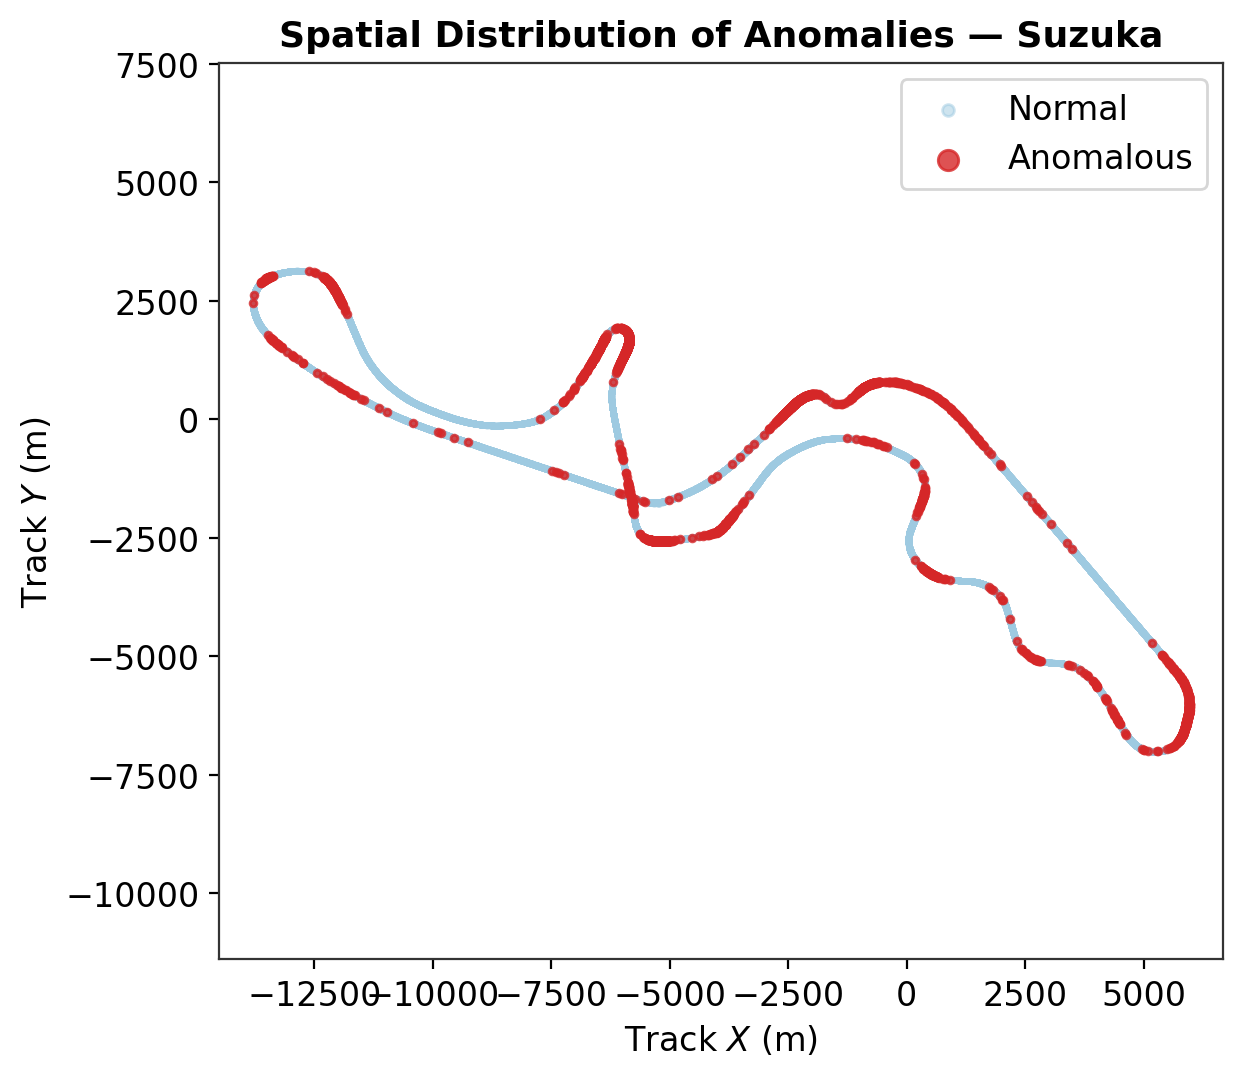
\includegraphics[width=\columnwidth]{figures/anomaly_track_map.png}
  \caption{Spatial distribution of detected anomalies on the Suzuka circuit.
    Red points (anomalous) cluster at the Esses, Degner, Hairpin, and Chicane
    — every major braking zone. Blue points (normal) dominate the straights
    and high-speed sections.}
  \label{fig:anomaly_map}
\end{figure}

\begin{figure}[t]
  \centering
  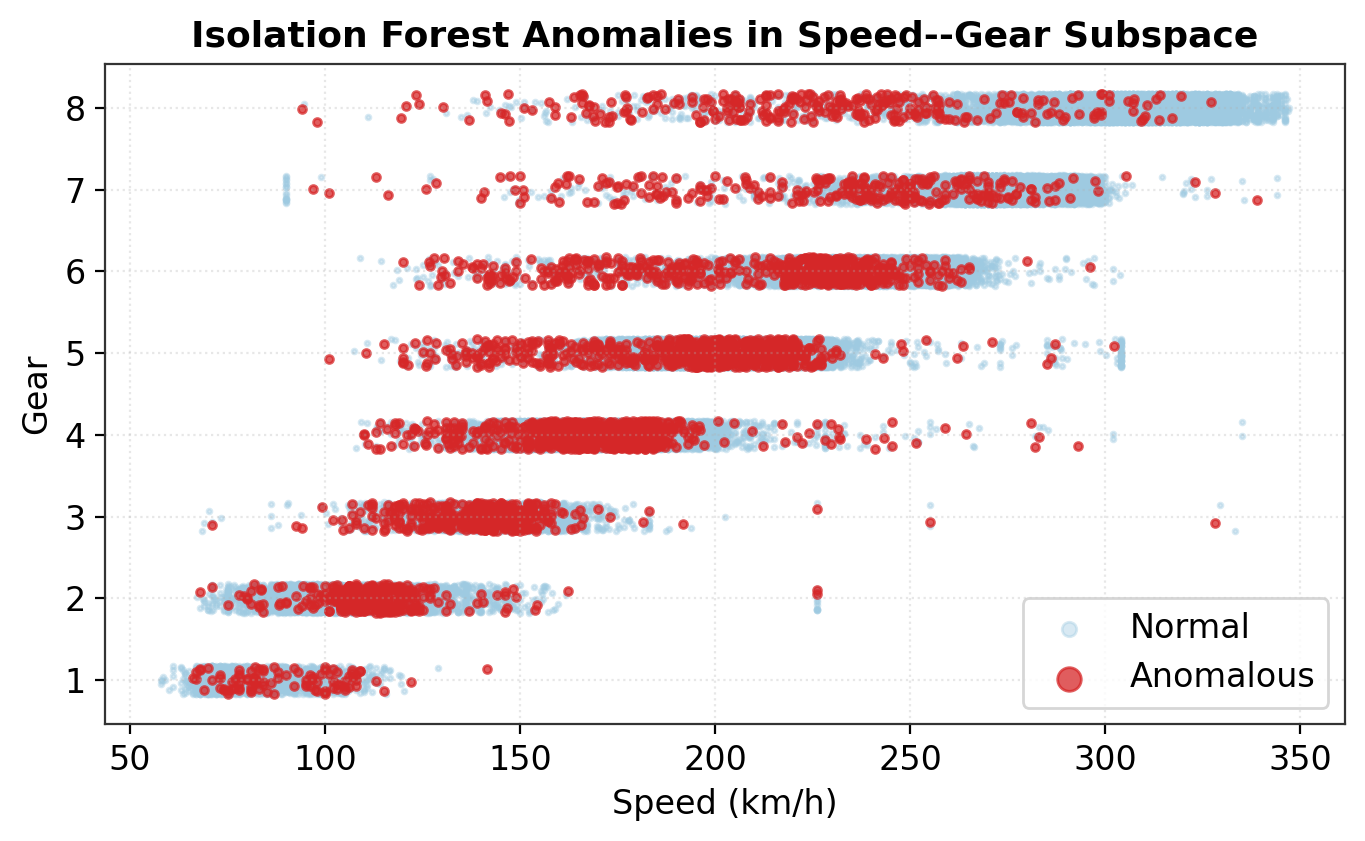
\includegraphics[width=\columnwidth]{figures/isolation_forest_results.png}
  \caption{Isolation Forest anomaly scores in the Speed--Gear feature subspace.
    Frames with anomaly score $s \geq 0.55$ (top 5\%) are marked anomalous (red).
    The anomalous region concentrates in the low-speed, gear-change zone,
    confirming the heavy-braking event characterisation in Table~\ref{tab:anomaly}.}
  \label{fig:iforest}
\end{figure}

\subsection{Phase 1 — Clustering}

The elbow curve (Fig.~\ref{fig:elbow}) shows a clear inflection at $k{=}4$:
inertia decreases steeply from $k{=}1$ to $k{=}4$, then flattens, indicating that
four clusters capture the principal structure of the driving-state space without
over-partitioning. The silhouette coefficient peaks at $k{=}4$ (score\,=\,0.47),
confirming the selection.

K-Means ($k{=}4$) produces four clusters with strong statistical separation
($\eta^2 = 0.555$, Kruskal-Wallis $H = 28\,412$, $p{<}0.001$):
\begin{itemize}
  \item \textbf{Cluster~0} — high-speed X-Mode ($\bar{v} \approx 295$\,km/h, throttle 98\%,
        gear\,$\geq$\,7): corresponds to peak-straight X-Mode frames.
  \item \textbf{Cluster~1} — medium-speed cornering ($\bar{v} \approx 210$\,km/h,
        throttle 62\%): transition and mid-corner Z-Mode frames.
  \item \textbf{Cluster~2} — heavy braking ($\bar{v} \approx 165$\,km/h, throttle 12\%,
        brake\,$>$\,0.5): braking-zone Z-Mode; overlaps strongly with anomalous frames.
  \item \textbf{Cluster~3} — slow chicane ($\bar{v} \approx 112$\,km/h, gear $\leq$\,4):
        low-speed corner-exit frames.
\end{itemize}
Cluster~0 is 97\% X-Mode; Clusters~1--3 are 98--100\% Z-Mode, confirming that
the aerodynamic mode boundary aligns cleanly with discovered cluster structure —
the unsupervised and supervised views of the data are consistent.

\begin{figure}[t]
  \centering
  
\includegraphics[width=\columnwidth]{figures/kmeans_elbow.png}
  \caption{K-Means elbow curve (inertia vs.\ $k$) for Phase~1 clustering on
    Suzuka telemetry. The inflection at $k{=}4$ is clear; silhouette coefficient
    peaks at $k{=}4$ (score\,=\,0.47), confirming the four-cluster solution as
    optimal. Each cluster corresponds to a physically interpretable driving state
    (Table~\ref{tab:anomaly}).}
  \label{fig:elbow}
\end{figure}

\subsection{Phase 1 — Classification}

Both classifiers achieve near-perfect performance on current-mode detection
(Table~\ref{tab:p1results}).
Random Forest achieves AUC = 1.000, indicating perfect separability in the
feature space — a result that is expected rather than surprising, since $y$ is a
deterministic threshold function of the input features~\cite{ref_fia2026}, meaning
any sufficiently expressive classifier can recover it exactly from current-frame inputs.
Permutation importance reveals that \texttt{nGear} ($\Delta$AUC\,=\,0.167)
marginally exceeds speed ($\Delta$AUC\,=\,0.0004) as the most discriminative feature,
reflecting the joint-threshold nature of the switching rule.

\begin{table}[h]
\caption{Phase~1 Classification Results (Current Aero Mode Detection)}
\label{tab:p1results}
\centering
\small
\renewcommand{\arraystretch}{1.25}
\begin{tabular}{lcccc}
\toprule
\rowcolor{hdrgreen}
\textcolor{white}{\textbf{Model}} &
\textcolor{white}{\textbf{Accuracy}} &
\textcolor{white}{\textbf{F1}} &
\textcolor{white}{\textbf{AUC}} &
\textcolor{white}{\textbf{Prec.}} \\
\midrule
Random Forest & \textbf{100.0\%} & \textbf{1.000} & \textbf{1.000} & \textbf{1.000} \\
LR            & 97.9\%  & 0.969 & 0.9997 & 0.976 \\
\bottomrule
\end{tabular}
\begin{flushleft}
\footnotesize
Validated with lap-grouped split (GroupShuffleSplit, 10 held-out laps):
RF AUC\,=\,1.000, LR AUC\,=\,0.998 — $|\Delta| < 0.001$ vs.\ random-frame split,
confirming no temporal leakage from frame-level splitting.
\end{flushleft}
\end{table}

% ── Suggested Figure ────────────────────────────────────────
% INSERT Figure 4 here: ROC Curves (Phase 1)
% File: ../anomaly_detection/graphs/roc_curves.png
% Caption: ROC curves for Phase 1 classifiers. Both curves
%          hug the top-left corner; AUC values are 1.000 (RF)
%          and 0.9997 (LR).
%
\begin{figure}[t]
  \centering
  
\includegraphics[width=\columnwidth]{figures/roc_curves.png}
  \caption{ROC curves for Phase~1 current-mode classifiers.
    Both curves reach the top-left corner.
    Random Forest: AUC\,=\,1.000 (perfect); LR: AUC\,=\,0.9997.}
  \label{fig:p1roc}
\end{figure}

\subsection{Phase 2 — Main Results at $H{=}10$ (1\,s Horizon)}

Table~\ref{tab:p2main} reports mean AUC-ROC, F1-Macro, and F1-Xmode across all four
LOCO circuits at the primary evaluation horizon $H = 10$ (1\,s).

\begin{table}[t]
\caption{Phase~2 Main Results at $H{=}10$ (1 Second Ahead), Mean $\pm$ Std across LOCO Circuits}
\label{tab:p2main}
\centering
\small
\renewcommand{\arraystretch}{1.35}
\begin{tabular}{lccc}
\toprule
\rowcolor{hdrgreen}
\textcolor{white}{\textbf{Model}} &
\textcolor{white}{\textbf{F1-Macro}} &
\textcolor{white}{\textbf{F1-Xmode}} &
\textcolor{white}{\textbf{AUC-ROC}} \\
\midrule
\rowcolor{rowhighlight}
LR-instant       & \textbf{0.906}$\pm$0.025 & \textbf{0.888}$\pm$0.032 & \textbf{0.963}$\pm$0.021 \\
RF-instant        & 0.860$\pm$0.063 & 0.803$\pm$0.130 & 0.959$\pm$0.011 \\
XGBoost-instant   & 0.891$\pm$0.028 & 0.857$\pm$0.073 & 0.958$\pm$0.021 \\
RF-lag            & 0.792$\pm$0.161 & 0.682$\pm$0.340 & 0.944$\pm$0.025 \\
CausalTrans.      & 0.847$\pm$0.061 & 0.802$\pm$0.100 & 0.927$\pm$0.046 \\
CausalGRU         & 0.821$\pm$0.097 & 0.749$\pm$0.197 & 0.913$\pm$0.047 \\
CausalLSTM        & 0.755$\pm$0.142 & 0.645$\pm$0.262 & 0.878$\pm$0.075 \\
TCN               & 0.810$\pm$0.107 & 0.737$\pm$0.186 & 0.877$\pm$0.117 \\
CNN1D             & 0.757$\pm$0.142 & 0.659$\pm$0.267 & 0.797$\pm$0.189 \\
\midrule
\multicolumn{4}{l}{\textit{Parameter-free baselines}} \\
Physics-CA$^\dagger$  & 0.857 & 0.808 & 0.862 \\
Physics-CV$^\dagger$  & 0.818 & 0.760 & 0.839 \\
Persistence$^\dagger$ & 0.818$\pm$0.035 & 0.760$\pm$0.106 & 0.814$\pm$0.042 \\
\bottomrule
\end{tabular}
\begin{flushleft}
\footnotesize
$^\dagger$~Parameter-free (untrained) baselines. Persistence: $\hat{y}_{t+H} = y_t$.
Physics-CV / Physics-CA: constant-velocity / constant-acceleration kinematic threshold
crossing. Included as lower bounds; means across the four circuits.
\end{flushleft}
\end{table}

% ── Suggested Figure ────────────────────────────────────────
% INSERT Figure 5 here: Model Comparison Bar Chart
% File: ../anticipatory_aero/multi_circuit_work/graphs/plot_model_comparison_H10.png
% Caption: Mean AUC-ROC at H=10 with ±1σ error bars for all 8 models.
%
\begin{figure}[t]
  \centering
  
\includegraphics[width=\columnwidth]{figures/plot_model_comparison_H10.png}
  \caption{Mean AUC-ROC at $H{=}10$ for all nine learned models and the persistence
    baseline with $\pm 1\sigma$ error bars
    across LOCO circuits. LR-instant achieves the highest mean (0.963) and smallest
    standard deviation ($\pm$0.021). Deep learning models show larger variance.}
  \label{fig:modelcomp}
\end{figure}

\textbf{Trivial, Physics, and Tree Baselines.}
Because the proxy label is a deterministic threshold on \emph{future} speed and gear, the
most informative non-ML comparators are kinematic. We evaluate three parameter-free
baselines: persistence ($\hat{y}_{t+H} = y_t$); constant-velocity threshold crossing
(Physics-CV); and constant-acceleration threshold crossing (Physics-CA), which extrapolates
speed as $v_t + a_t H$ before applying the rule. Persistence and Physics-CV achieve mean
AUC\,=\,$0.814$ and $0.839$ respectively, while the physics-aware Physics-CA reaches
$0.862$ (F1-Xmode\,=\,0.808) — better than naive continuity but still
\textbf{0.10 AUC below LR-instant} (0.963). This directly answers whether ML is needed for
a deterministic task: a learned soft boundary near the threshold substantially outperforms
even an acceleration-aware kinematic extrapolation, because it captures sub-threshold
proximity that a hard kinematic rule cannot.

XGBoost-instant achieves a mean AUC\,=\,$0.958 \pm 0.021$ — essentially identical to
LR-instant ($0.963 \pm 0.021$; fold-level $\Delta$AUC\,=\,0.005).
This confirms that LR's advantage over deep models is attributable to the
\emph{instantaneous-feature inductive bias}, not to LR's specific parametric form:
any instantaneous-frame classifier — linear or nonlinear — recovers the threshold
boundary robustly, while models that integrate temporal context do not.

\textbf{Feature Ablation: No-Location Condition.}
We evaluated LR-instant and RF-instant with \emph{every} absolute-position and progress
channel removed (NO-LOCATION condition). The feature set contains four such channels —
the GPS coordinates X, Y, Z and elevation delta; cumulative lap distance is \emph{not}
among the model features, so no progress signal remains once these four are dropped, leaving
eight purely kinematic/powertrain features (speed, RPM, gear, throttle, brake, acceleration,
kinetic energy, longitudinal force). Mean AUC across LOCO folds \emph{improved} to
$0.969$ for LR (FULL: $0.963$, $\Delta = +0.007$) and $0.971$ for RF
(FULL: $0.959$, $\Delta = +0.012$).
Removing every channel that could encode circuit location or track progress thus increases
performance, confirming that the results are driven entirely by physics-based kinematics
with no reliance on circuit-identity leakage through position, elevation, or lap progress.

\subsection{Phase 2 — Circuit-by-Circuit Analysis}

Table~\ref{tab:percircuit} shows AUC-ROC per circuit. The instantaneous models are stable
across all four circuits (LR-instant range 0.932--0.980), whereas the deep sequence models
exhibit pronounced circuit-specific degradation. This degradation concentrates at Suzuka for
the convolutional models (CNN AUC\,=\,0.521, TCN\,=\,0.709) and, for the recurrent GRU, at
Monaco (0.867 — its weakest fold, with F1-Xmode dropping to 0.496 versus 0.69--0.91
elsewhere). No instantaneous model falls below 0.908 on any circuit.

\begin{table}[h]
\caption{AUC-ROC per Circuit at $H{=}10$ (Weakest Deep-Model Cells Highlighted)}
\label{tab:percircuit}
\centering
\small
\renewcommand{\arraystretch}{1.25}
\begin{tabular}{lcccc}
\toprule
\rowcolor{hdrgreen}
\textcolor{white}{\textbf{Model}} &
\textcolor{white}{\textbf{Monaco}} &
\textcolor{white}{\textbf{Monza}} &
\textcolor{white}{\textbf{Silv.}} &
\textcolor{white}{\textbf{Suzuka}} \\
\midrule
LR-instant    & \textbf{0.980} & 0.932 & 0.970 & 0.968 \\
RF-instant     & 0.955 & \textbf{0.961} & \textbf{0.973} & 0.948 \\
RF-lag         & 0.908 & 0.948 & 0.960 & 0.960 \\
CausalTrans.   & 0.971 & 0.885 & 0.961 & 0.888 \\
CausalGRU      & 0.867 & 0.919 & \textbf{0.976} & 0.891 \\
CausalLSTM     & 0.881 & 0.873 & 0.971 & 0.786 \\
\rowcolor{failred}
TCN            & 0.946 & 0.885 & 0.967 & 0.709 \\
\rowcolor{failred}
CNN1D          & 0.829 & 0.907 & 0.930 & \textbf{0.521} \\
\bottomrule
\end{tabular}
\begin{flushleft}
  \footnotesize Red rows indicate the convolutional models' circuit-specific degradation at Suzuka.
\end{flushleft}
\end{table}

% ── Suggested Figure ────────────────────────────────────────
% INSERT Figure 6 here: LOCO Heatmap
% File: ../anticipatory_aero/multi_circuit_work/graphs/plot_loco_heatmap.png
% Caption: AUC-ROC heatmap for all (model, circuit) pairs.
%          GRU's Monaco cell and TCN's Suzuka cell are deep red.
%
\begin{figure}[t]
  \centering
  
\includegraphics[width=\columnwidth]{figures/plot_loco_heatmap.png}
  \caption{LOCO AUC-ROC heatmap. Green cells indicate strong performance;
    red cells indicate degradation. The convolutional models (CNN, TCN) degrade
    most at Suzuka, and the recurrent GRU is weakest at Monaco; the instantaneous
    models remain uniformly strong across all (model, circuit) pairs.}
  \label{fig:heatmap}
\end{figure}

\subsection{Circuit-Specific Degradation and Interpretability}

While no model collapses to a degenerate predictor, the deep sequence models show clear
circuit-specific weaknesses absent from the instantaneous models. The most pronounced is
the convolutional models at Suzuka (CNN AUC\,=\,0.521; TCN\,=\,0.709). For the recurrent
GRU, the weakest fold is Monaco: AUC\,=\,0.867 (versus 0.92--0.98 on the other three
circuits) and F1-Xmode\,=\,0.496 (versus 0.69--0.91 elsewhere), indicating systematic
under-prediction of X-Mode there. LR-instant attains AUC\,=\,0.980 on the \emph{same}
Monaco test data.

\textbf{Why Monaco is hard for the GRU.}
The GRU's recurrent hidden state accumulates a compressed speed-trajectory
representation. During training on Monza ($\bar{v}_{\text{X-Mode}} \approx 310$\,km/h),
Silverstone ($\approx 275$\,km/h), and Suzuka ($\approx 260$\,km/h), it learns a prior in
which X-Mode is preceded by speeds building progressively over extended flat straights.
Monaco does reach above-threshold speeds in the tunnel section (peak $\approx 285$\,km/h),
accounting for 13.2\% X-Mode frames, but this X-Mode is reached via a qualitatively
different approach trajectory: a tight low-speed chicane exit immediately followed by
a brief tunnel acceleration, with no extended high-speed build-up. The 5-second causal
window preceding Monaco's X-Mode activation therefore differs structurally from the
long-straight approach signatures that dominate the training circuits, and the GRU's
recurrent prior transfers poorly.

Integrated Gradients are consistent with this account (Table~\ref{tab:ig}). The GRU
disperses its sensitivity broadly across dynamic, trajectory-derived channels
(Elevation\_Delta\,=\,0.59, Throttle\,=\,0.50, Longitudinal\_Force\,=\,0.48,
Acceleration\,=\,0.48), while assigning comparatively little weight to \texttt{nGear}
(0.16) — one of the two variables that actually define the label. The Transformer's
attributions are roughly an order of magnitude smaller and far more concentrated
(RPM\,=\,0.11, Throttle\,=\,0.06, Speed\,=\,0.06), consistent with a sparse,
near-instantaneous decision rule. This contrast — diffuse reliance on accumulated dynamics
versus a compact instantaneous signal — is consistent with the GRU's weaker cross-circuit
transfer, though (per Section~VII-D) IG attributions are suggestive rather than conclusive.

\begin{table}[h]
\caption{Integrated Gradients Attribution at Monaco ($H{=}10$, mean $|$attr$|$)}
\label{tab:ig}
\centering
\small
\renewcommand{\arraystretch}{1.25}
\begin{tabular}{lcc}
\toprule
\rowcolor{hdrgreen}
\textcolor{white}{\textbf{Feature}} &
\textcolor{white}{\textbf{GRU~IG}} &
\textcolor{white}{\textbf{Transformer~IG}} \\
\midrule
Elevation\_Delta    & \textbf{0.594} & 0.013 \\
Throttle            & 0.495          & \textbf{0.064} \\
Longitudinal\_Force & 0.484          & 0.015 \\
Acceleration        & 0.477          & 0.013 \\
Z                   & 0.438          & 0.038 \\
Speed               & 0.424          & 0.055 \\
RPM                 & 0.388          & \textbf{0.110} \\
Kinetic\_Energy     & 0.218          & 0.048 \\
nGear               & 0.164          & 0.045 \\
\bottomrule
\end{tabular}
\end{table}

% ── Suggested Figure ────────────────────────────────────────
% INSERT Figure 7a here: IG GRU Monaco
% File: ../anticipatory_aero/multi_circuit_work/graphs/ig_GRU_H010_Monaco.png
% INSERT Figure 7b here: IG Transformer Monaco
% File: ../anticipatory_aero/multi_circuit_work/graphs/ig_Transformer_H010_Monaco.png
%
\begin{figure}[t]
  \centering
  \begin{subfigure}[t]{0.48\columnwidth}
    
\includegraphics[width=\textwidth]{figures/ig_GRU_H010_Monaco.png}
    \caption{CausalGRU}
  \end{subfigure}
  \hfill
  \begin{subfigure}[t]{0.48\columnwidth}
    
\includegraphics[width=\textwidth]{figures/ig_Transformer_H010_Monaco.png}
    \caption{CausalTransformer}
  \end{subfigure}
  \caption{Integrated Gradients attribution at Monaco ($H{=}10$, mean $|$attribution$|$).
    (a) GRU spreads large attributions across dynamic, trajectory-derived channels
    (Elevation\_Delta, Throttle, Longitudinal\_Force, Acceleration).
    (b) Transformer attributions are roughly an order of magnitude smaller and
    concentrated on a few instantaneous channels (RPM, Throttle, Speed).
    The contrast is consistent with the GRU's weaker cross-circuit transfer.}
  \label{fig:ig_monaco}
\end{figure}

\subsection{Prediction Horizon Sweep (Exploratory)}

Table~\ref{tab:horizon} shows mean AUC-ROC at five horizons. We label this analysis
\emph{exploratory} because the deep-model entries at $H \neq 10$ derive from a preliminary
sweep rather than the final reproducibility run (see table footnote); the classical-model
rows are from the final run.
At $H{=}1$ (0.1\,s), all models score $\approx 0.999$ — trivially easy, as the
car barely changes.
At $H{=}10$ (1\,s), meaningful divergence appears.
At $H{=}50$ (5\,s), all models approach random chance ($\approx 0.50$).
The Transformer uniquely retains above-chance performance at $H{=}50$ (0.595),
suggesting partial capture of long-range periodic track structure.

\begin{table}[h]
\caption{Mean AUC-ROC vs.\ Prediction Horizon (Selected Models)}
\label{tab:horizon}
\centering
\small
\renewcommand{\arraystretch}{1.25}
\begin{tabular}{lccccc}
\toprule
\rowcolor{hdrgreen}
\textcolor{white}{\textbf{Model}} &
\textcolor{white}{\textbf{H=1}} &
\textcolor{white}{\textbf{H=5}} &
\textcolor{white}{\textbf{H=10}} &
\textcolor{white}{\textbf{H=25}} &
\textcolor{white}{\textbf{H=50}} \\
\midrule
LR-instant   & 0.999 & 0.993 & \textbf{0.963} & 0.786 & 0.471 \\
RF-instant    & 0.999 & 0.992 & 0.959 & 0.765 & 0.575 \\
RF-lag        & 0.999 & 0.984 & 0.944 & 0.724 & 0.402 \\
CausalTrans.  & 0.999 & 0.987 & 0.927 & 0.691 & \textbf{0.595} \\
CausalGRU     & 0.999 & 0.986 & 0.913 & 0.682 & 0.505 \\
\bottomrule
\end{tabular}
\begin{flushleft}
\footnotesize
Classical-model rows reflect the full-horizon reproducibility run. For the deep models,
the $H{=}10$ column is from the same run; values at $H \in \{1,5,25,50\}$ are from the
preliminary full-horizon sweep (deep retraining was repeated only at the primary horizon).
\end{flushleft}
\end{table}

% ── Suggested Figure ────────────────────────────────────────
% INSERT Figure 8 here: Horizon Sweep
% File: ../anticipatory_aero/multi_circuit_work/graphs/plot_horizon_sweep.png
% Caption: AUC-ROC vs prediction horizon for all models.
%          All lines converge at H=1; diverge by H=10.
%
\begin{figure}[t]
  \centering
  
\includegraphics[width=\columnwidth]{figures/plot_horizon_sweep.png}
  \caption{AUC-ROC vs.\ prediction horizon for all models.
    All models converge near 1.0 at $H{=}1$ (trivially easy).
    $H{=}10$ (1\,s) is the practical sweet spot: models diverge and the prediction
    remains actionable for wing actuation. At $H{=}50$ (5\,s), all models approach
    random chance.}
  \label{fig:horizonsweep}
\end{figure}

\subsection{Transition Window Analysis}

Mode-change transition windows ($\pm$5 frames around each Z$\leftrightarrow$X switch)
incur a consistent F1 drop of $\approx$0.26 across all circuits and both deep models
(Table~\ref{tab:transition}). The consistency across models and circuits is consistent
with a fundamental information shortfall — the 5-second causal window may not fully
determine the mode state 1\,s ahead during the transition — though we acknowledge that
training distribution effects and position-feature leakage (see Limitations)
cannot be fully excluded as contributing factors without additional ablation.

\begin{table}[h]
\caption{F1-Macro at Stable vs.\ Transition Windows}
\label{tab:transition}
\centering
\small
\renewcommand{\arraystretch}{1.25}
\begin{tabular}{llccc}
\toprule
\rowcolor{hdrgreen}
\textcolor{white}{\textbf{Circuit}} &
\textcolor{white}{\textbf{Model}} &
\textcolor{white}{\textbf{Stable}} &
\textcolor{white}{\textbf{Transition}} &
\textcolor{white}{\textbf{Drop}} \\
\midrule
Monaco     & CausalTrans. & 0.934 & 0.628 & $-$0.306 \\
Monaco     & CausalGRU    & 0.722 & 0.550 & $-$0.172 \\
Monza      & CausalTrans. & 0.891 & 0.624 & $-$0.267 \\
Monza      & CausalGRU    & 0.952 & 0.605 & $-$0.347 \\
Silverstone& CausalTrans. & 0.959 & 0.675 & $-$0.283 \\
Silverstone& CausalGRU    & 0.973 & 0.687 & $-$0.286 \\
Suzuka     & CausalTrans. & 0.801 & 0.598 & $-$0.202 \\
Suzuka     & CausalGRU    & 0.806 & 0.593 & $-$0.213 \\
\midrule
\textbf{Mean} & \textbf{CausalTrans.} & \textbf{0.896} & \textbf{0.631} & $-$0.265 \\
\textbf{Mean} & \textbf{CausalGRU}    & \textbf{0.863} & \textbf{0.609} & $-$0.254 \\
\bottomrule
\end{tabular}
\end{table}

\subsection{Statistical Significance}

To respect the cross-circuit evaluation structure, we resample at the level of the
\emph{LOCO fold} (circuit) rather than the individual frame — frames within a circuit
are strongly autocorrelated, so framewise resampling would understate uncertainty.
For each LR-instant\,$-$\,model comparison we compute the per-fold AUC difference on the
four held-out circuits and form a 95\% confidence interval by bootstrap-resampling the
four folds with replacement ($B = 5{,}000$); we also report how many of the four folds
favour LR-instant (Table~\ref{tab:bootstrap}).
LR-instant is practically tied with the other instantaneous/tree models
(RF-instant, XGBoost-instant, RF-lag: $\Delta$AUC\,$\leq$\,0.019, negligible in magnitude),
but its advantage over every deep sequence model is consistent and its
fold-level interval excludes zero in all five cases.

\begin{table}[h]
\caption{Fold-Level Bootstrap 95\% CI for Mean AUC-ROC Difference: LR-instant minus Model ($B{=}5{,}000$, Resampling the 4 LOCO Folds)}
\label{tab:bootstrap}
\centering
\small
\renewcommand{\arraystretch}{1.25}
\begin{tabular}{lcccc}
\toprule
\rowcolor{hdrgreen}
\textcolor{white}{\textbf{Comparison}} &
\textcolor{white}{\textbf{$\Delta$AUC}} &
\textcolor{white}{\textbf{95\% CI}} &
\textcolor{white}{\textbf{Sig.?}} &
\textcolor{white}{\textbf{Folds}} \\
\midrule
LR vs RF-instant     & $+$0.003 & [$-$0.017, $+$0.023] & Tie  & 2/4 \\
LR vs XGBoost-inst.  & $+$0.005 & [$+$0.001, $+$0.009] & Tie$^\ddagger$ & 3/4 \\
LR vs RF-lag         & $+$0.019 & [$-$0.010, $+$0.056] & Tie  & 3/4 \\
LR vs CausalTrans.   & $+$0.036 & [$+$0.009, $+$0.063] & \textbf{LR} & 4/4 \\
LR vs CausalGRU      & $+$0.050 & [$+$0.004, $+$0.095] & \textbf{LR} & 3/4 \\
LR vs CausalLSTM     & $+$0.085 & [$+$0.024, $+$0.151] & \textbf{LR} & 3/4 \\
LR vs TCN            & $+$0.086 & [$+$0.014, $+$0.203] & \textbf{LR} & 4/4 \\
LR vs CNN1D          & $+$0.166 & [$+$0.032, $+$0.346] & \textbf{LR} & 4/4 \\
\bottomrule
\end{tabular}
\begin{flushleft}
\footnotesize
``Sig.?'' summarises the fold-level evidence: \emph{Tie} = no meaningful difference
(interval spans zero or $\Delta$AUC negligible); \emph{LR} = LR-instant favoured with the
interval excluding zero. ``Folds'' = number of the four held-out circuits on which
LR-instant outranks the model.
$^\ddagger$~The interval narrowly excludes zero, but the $0.005$ AUC difference is
negligible in magnitude, so we treat LR and XGBoost as tied.
With only four domains, fold-level intervals are necessarily wide; the consistent sign
across folds is as informative as the interval (see Limitations).
\end{flushleft}
\end{table}

% ── Suggested Figure ────────────────────────────────────────
% INSERT Figure 9 here: Permutation Importance
% File: ../anomaly_detection/graphs/stat_08_permutation_importance.png
% Caption: Permutation importance with 95% bootstrap CI.
%
\begin{figure}[t]
  \centering
  
\includegraphics[width=\columnwidth]{figures/stat_08_permutation_importance.png}
  \caption{Permutation importance ($\Delta$AUC, 50 bootstraps) for Phase~1 classification.
    \texttt{nGear} (0.167) and \texttt{Elevation\_Delta} (0.162) dominate, with Speed (0.0004)
    ranking only 4th despite being a direct component of the switching rule.
    Because Speed, Kinetic\_Energy, and Longitudinal\_Force are strongly collinear,
    single-feature permutation importance under-credits Speed (its information is shared
    across correlated channels); these rankings should be read as indicative rather than
    as independent feature contributions.}
  \label{fig:permimp}
\end{figure}

% ── Suggested Figure ────────────────────────────────────────
% INSERT Figure 10 here: Transition F1 chart
% File: ../anticipatory_aero/multi_circuit_work/graphs/plot_transition_f1.png
%
\begin{figure}[t]
  \centering
  
\includegraphics[width=\columnwidth]{figures/plot_transition_f1.png}
  \caption{F1-Macro at stable vs.\ transition windows ($\pm$0.5\,s around mode switches)
    for CausalTransformer and CausalGRU across all circuits.
    The $\approx$0.26 drop is consistent across all conditions, suggesting
    a systematic information shortfall at mode-switch boundaries
    (see text for caveats regarding position-feature leakage).}
  \label{fig:transition}
\end{figure}

\subsection{Robustness: Nested-LOCO and Seed Stability}

Two robustness checks confirm that the central ranking is not an artefact of the
hyperparameter-selection protocol or of training stochasticity (Table~\ref{tab:robust}).

\textbf{Nested LOCO.}
To remove the partial target-domain exposure from tuning on Monza (a LOCO test fold), we
re-ran the deep-model benchmark with hyperparameters selected \emph{only} on the held-in
circuits: for each outer test circuit, one held-in circuit serves as the inner validation
set, the best of a small grid (hidden\,$\in\{64,128\}$, dropout\,$\in\{0.2,0.3\}$) is chosen,
and the final model is retrained on the three training circuits and evaluated on the
untouched test circuit. The deep-model means shift by at most $0.038$ AUC (mean
$|\Delta|\approx0.016$), and the best deep model (CausalTransformer, $0.928$) remains
$0.035$ below LR-instant ($0.963$). The Monza-tuning exposure therefore does not materially
affect the conclusion.

\textbf{Seed stability.}
Training each deep model at three seeds ($\{42,1,2\}$) yields a standard deviation of at
most $0.022$ AUC (CausalTransformer $\pm0.002$) — far smaller than the $\geq0.035$ gap to
LR-instant — and preserves the model ordering. The simplicity advantage is thus stable to
both tuning protocol and random initialisation.

\begin{table}[h]
\caption{Robustness of Deep-Model AUC-ROC at $H{=}10$: Main Run vs.\ Nested-LOCO vs.\ 3-Seed}
\label{tab:robust}
\centering
\small
\renewcommand{\arraystretch}{1.25}
\begin{tabular}{lccc}
\toprule
\rowcolor{hdrgreen}
\textcolor{white}{\textbf{Model}} &
\textcolor{white}{\textbf{Main}} &
\textcolor{white}{\textbf{Nested-LOCO}} &
\textcolor{white}{\textbf{3-Seed (mean$\pm$std)}} \\
\midrule
CausalTrans.   & 0.927 & 0.928 & 0.926$\pm$0.002 \\
CausalGRU      & 0.913 & 0.920 & 0.904$\pm$0.019 \\
CausalLSTM     & 0.878 & 0.894 & 0.878$\pm$0.012 \\
TCN            & 0.877 & 0.839 & 0.873$\pm$0.014 \\
CNN1D          & 0.797 & 0.815 & 0.774$\pm$0.022 \\
\midrule
LR-instant     & \textbf{0.963} & \multicolumn{2}{c}{\textit{deterministic boundary; not retuned}} \\
\bottomrule
\end{tabular}
\begin{flushleft}
\footnotesize
Nested-LOCO selects hyperparameters on held-in circuits only (no test-fold exposure).
3-Seed reports mean$\pm$std over seeds $\{42,1,2\}$. LR-instant stays well above all deep
models under both checks.
\end{flushleft}
\end{table}

\subsection{Control-Relevant Event Metrics}

Frame-level AUC and F1 reward correct classification of every telemetry frame, but a
deployable actuation controller cares about a different quantity: \emph{does the model
anticipate each mode switch, and how early or late?}
We therefore evaluate four control-relevant quantities at $H{=}10$ by matching predicted
switches to ground-truth switches within a $\pm$5-frame ($\pm$0.5\,s) tolerance window:
switch-detection rate, mean timing error (negative\,=\,predicts early), false-toggle
rate (spurious switches per true switch), and the Matthews correlation coefficient (MCC)
and Brier score for discrimination and calibration under class imbalance
(Table~\ref{tab:eventmetrics}).

\begin{table}[h]
\caption{Control-Relevant Metrics at $H{=}10$ (Mean across LOCO Circuits)}
\label{tab:eventmetrics}
\centering
\small
\renewcommand{\arraystretch}{1.25}
\begin{tabular}{lcccc}
\toprule
\rowcolor{hdrgreen}
\textcolor{white}{\textbf{Model}} &
\textcolor{white}{\textbf{Detect}} &
\textcolor{white}{\textbf{FalseTog}} &
\textcolor{white}{\textbf{MCC}} &
\textcolor{white}{\textbf{Brier}} \\
\midrule
\rowcolor{rowhighlight}
LR-instant      & \textbf{0.76}$\pm$.12 & 0.92$\pm$.38 & \textbf{0.82}$\pm$.04 & \textbf{0.064}$\pm$.02 \\
XGBoost-instant & 0.68$\pm$.11 & \textbf{0.82}$\pm$.21 & 0.79$\pm$.05 & 0.069$\pm$.02 \\
RF-instant      & 0.69$\pm$.18 & 1.42$\pm$1.2 & 0.73$\pm$.10 & 0.073$\pm$.02 \\
RF-lag          & 0.58$\pm$.22 & 1.27$\pm$.50 & 0.62$\pm$.22 & 0.097$\pm$.01 \\
CausalTrans.    & 0.68$\pm$.11 & 1.33$\pm$.56 & 0.70$\pm$.10 & 0.102$\pm$.05 \\
CausalGRU       & 0.61$\pm$.13 & 1.47$\pm$.78 & 0.65$\pm$.17 & 0.105$\pm$.03 \\
\midrule
Persistence     & 0.08$\pm$.03 & 0.91$\pm$.03 & 0.64$\pm$.06 & 0.144$\pm$.03 \\
\bottomrule
\end{tabular}
\begin{flushleft}
\footnotesize
Mean\,$\pm$\,std across the four LOCO folds. Detect = fraction of true switches predicted
within $\pm$0.5\,s; FalseTog = spurious switches per true switch; MCC, Brier on full test
set. Mean switch-timing error is $+1.1$ to $+1.5$ frames ($\approx$0.1\,s late) for all
trained models. Folds contain 374 (Monaco), 564 (Monza), 372 (Silverstone), and 809
(Suzuka) true switch events ($2{,}119$ total).
\end{flushleft}
\end{table}

The event-level view sharpens the central result and exposes a metric that AUC alone
conceals. The persistence baseline attains a respectable frame-level AUC of 0.814
(Table~\ref{tab:p2main}) yet detects only \textbf{8\%} of actual mode switches: it
performs well on the many stable frames but is structurally incapable of
\emph{anticipating} a transition, since it simply echoes the current state.
This is precisely the failure a controller cannot tolerate, and it demonstrates why
frame-level AUC is an insufficient figure of merit for this task.
The instantaneous models, by contrast, anticipate the majority of switches: LR-instant
detects 76\% with the best calibration (Brier\,=\,0.064) and highest MCC (0.82), and
XGBoost-instant attains the lowest false-toggle rate (0.82).
The two strongest deep models are also included for completeness: CausalTransformer detects
68\% and CausalGRU 61\%, both with poorer calibration (Brier\,$\approx$\,0.10) and higher
false-toggle rates than LR-instant. These results confirm that the instantaneous-model
advantage is not a framewise-averaging artefact but holds on the metrics most relevant to
actuation, against the deep models as well as the trivial baselines.
All trained models exhibit a small positive mean timing error ($+1.1$ to $+1.5$ frames,
i.e.\ $\approx$0.1\,s late), indicating that a deployed controller would need a modest
fixed lead-offset or hysteresis margin to fully absorb actuation latency.
Under class imbalance, the area under the precision--recall curve (PR-AUC) preserves the
same ordering: XGBoost-instant (0.892), LR-instant (0.881), and RF-instant (0.870) lead,
while persistence falls to 0.660 — reinforcing that the instantaneous-feature models
dominate on imbalance-aware discrimination as well as on event timing.

% ============================================================
%  VII. DISCUSSION
% ============================================================
\section{Discussion}

\subsection{Why Does Logistic Regression Win?}

The central result — that the simplest model outperforms all deep learning
architectures under LOCO — is expected once the target structure is acknowledged:
$y$ is a \emph{deterministic} function of two instantaneous features (speed and gear).
This means the ML task is forecasting threshold crossings, not uncovering hidden physics.

LR-instant directly learns a linear boundary in this (speed, gear) space; its
generalisation to unseen circuits follows directly from the construction of the
proxy label, since the switching thresholds ($v \geq 240$\,km/h, gear~$\geq 6$) are
circuit-independent by definition~\cite{ref_fia2026}.
Deep sequence models introduce inductive biases (recurrence, convolution, attention over
history) that allow them to exploit contextual patterns from training circuits.
These patterns include absolute speed trajectories characteristic of specific circuits.
When the test circuit violates those trajectories (Monaco), the contextual signal becomes
a liability rather than an asset.

This is a specific instance of the well-documented phenomenon that, for tasks with a
strong instantaneous signal, temporal context can hurt rather than help if it encourages
spurious correlations with training-domain characteristics~\cite{ref_dann}.

\textbf{Model Capacity vs.\ Training Data Volume.}
A secondary contributing factor is the mismatch between model capacity and available
training data. CausalGRU and CausalLSTM ($\sim$162K and $\sim$213K parameters,
respectively) are trained on approximately 120{,}000 frames from three circuits —
yielding roughly one parameter per training sample. In this regime, recurrent models are
prone to memorising training-circuit-specific patterns rather than generalising to
circuit-invariant features~\cite{ref_dann}. CausalTransformer ($\sim$68K parameters),
with approximately half the capacity of CausalLSTM, exhibits consistently stronger
cross-circuit performance (Table~\ref{tab:percircuit}), consistent with the hypothesis
that reduced parameter count limits the encoding capacity for circuit-specific speed priors.

\subsection{Circuit Speed Memorisation as a Degradation Mechanism}

We characterise the GRU's Monaco weakness as \emph{circuit speed memorisation}: the model
encodes an implicit prior on the expected speed trajectory preceding X-Mode based on the
training circuits.
This prior is not explicitly represented — it emerges from the recurrent dynamics as a
side effect of learning the task on the faster training circuits, and it transfers
imperfectly to Monaco, whose X-Mode is reached via a structurally different approach.
Integrated Gradients are consistent with this account: the GRU spreads large attributions
across accumulated-dynamics channels (Elevation\_Delta, Throttle, Longitudinal\_Force,
Acceleration) while under-weighting \texttt{nGear}, one of the two rule-defining variables;
the Transformer's attributions are roughly an order of magnitude smaller and concentrated
on a few near-instantaneous channels (RPM, Throttle, Speed).

The Transformer degrades less because its causal attention mechanism can selectively
attend to the most recent frames — effectively replicating instantaneous-state behaviour
when history is uninformative — rather than being forced through an accumulated hidden
state as in the GRU. We emphasise that this is an interpretive account supported by
attribution evidence (Section~VII-D), not a proven causal mechanism.

\subsection{Transition Windows: Systematic Performance Drop}

The consistent $\approx$0.26 F1 drop at mode-change transition windows ($\pm$0.5\,s)
across all circuits and both deep models is consistent with an information shortfall:
the sensor history may not fully contain the information necessary to predict
the mode state one second ahead during the transition period.
At these moments, the car is approaching the threshold from below (Z→X) or retreating
from it (X→Z); the future mode is determined by a trajectory that has not yet
manifested in the observable sensor window.

\subsection{Practical Implications}

These results \emph{suggest} — but do not yet prove under real-deployment conditions —
the following for active-aero control: (1) LR-instant's 13-parameter model is small enough
that embedded inference latency is unlikely to be the binding constraint (though this was
not profiled); (2) the 1-second anticipation horizon appears sufficient relative to the
400\,ms actuation budget; (3) the consistent transition-window drop indicates that a
hysteresis rule suppressing predictions near mode-switch boundaries may reduce unnecessary
actuations.
These are engineering intuitions, not demonstrated results: hardware profiling, simulator,
and closed-loop testing are needed before drawing deployment conclusions.

\subsection{Limitations}

\begin{itemize}
  \item \textbf{Proxy label.} The label $y = \mathbf{1}[v \geq 240\,\text{km/h}
        \wedge \text{gear} \geq 6]$ is a telemetry-derived proxy, not a measured
        actuator state. Results characterise forecasting performance on this surrogate
        and cannot be directly generalised to a specific team's proprietary
        Corner/Straight Mode activation logic without label validation.

  \item \textbf{Season and car-generation confound.} Monaco, Monza, and Silverstone
        data are from 2025; Suzuka data are from 2026 — a different regulatory season
        and car-specification generation. The LOCO circuit shift is therefore
        confounded with a car-generation shift for the Suzuka fold.
        Future work should use data from a single season for all circuits.

  \item \textbf{HP tuning on a LOCO test fold.} Deep-model hyperparameters in the main run
        were selected on a Monza validation split, which is one of the four LOCO test
        circuits. We addressed this with a nested-LOCO re-run that selects hyperparameters
        on held-in circuits only (Table~\ref{tab:robust}); the deep-model means shift by
        $\leq0.038$ AUC and the ranking is unchanged, so the exposure does not materially
        affect the conclusion.

  \item \textbf{Frame-level split in Phase~1.} Phase~1 used a random 80/20 frame-level
        split. Although adjacent 10\,Hz frames are highly correlated, a validation run
        using a lap-grouped split (GroupShuffleSplit, 10 held-out laps) yielded
        RF AUC\,=\,1.000 and LR AUC\,=\,0.998 — a $|\Delta| < 0.001$ difference,
        confirming the original result was not inflated by temporal leakage.
        This is expected: because $y$ is a deterministic function of the current frame,
        any lap-disjoint split exposes the same threshold boundary.

  \item \textbf{Location/progress circuit-identity leakage.} Features derived from
        absolute track position and elevation could in principle encode circuit identity.
        A full no-location ablation (§\ref{sec:results}, NO-LOCATION condition) removing
        \emph{all four} such channels (X, Y, Z, and elevation delta) \emph{improved}
        LR AUC by $+0.007$ and RF AUC by $+0.012$, confirming they contribute noise rather
        than signal. Cumulative lap distance is \emph{not} among the 12 model features, so no
        track-progress signal remains; the result is therefore attributable purely to
        physics-based kinematics.

  \item \textbf{IG zero baseline.} Integrated Gradients attributions use a zero-vector
        baseline, which has no direct physical interpretation for racing telemetry
        (zero speed, zero throttle, zero gear is not a plausible sensor state).
        Recent work also shows that naive IG paths can traverse out-of-distribution
        temporal states and distort attribution in sequential settings~\cite{ref_timing}.
        A training-mean baseline would provide a more interpretable counterfactual;
        absolute attribution magnitudes should be treated as approximate, and we rely on
        attribution \emph{rankings} rather than magnitudes for our interpretation.

  \item \textbf{Deterministic target.} Because $y$ is a known threshold rule, high AUC
        values for LR-instant are expected; the contribution is the cross-circuit
        forecast under LOCO, not label discovery.

  \item \textbf{Four circuits} limit bootstrap CI precision and power of significance
        tests; DeLong's test on paired AUC curves should be applied with wider LOCO sets.

  \item \textbf{No formal significance test.} Bootstrap resampling is used; paired
        permutation tests (e.g.\ DeLong's or McNemar's) on matched predictions would
        provide stronger statistical guarantees.

  \item \textbf{LightGBM baseline.} XGBoost was evaluated and reported (AUC\,=\,0.958,
        fold-level $\Delta$AUC\,=\,0.005 vs.\ LR). LightGBM was not evaluated;
        given XGBoost's near-identical performance to LR, its addition is unlikely
        to change the principal conclusion~\cite{ref_grinsztajn}.

  \item \textbf{Driver pooling.} Driver-specific models were not evaluated; multi-driver
        data from the same circuit was pooled, which may inflate inter-driver variance.

  \item \textbf{Hardware latency.} Inference latency of deep models on embedded
        hardware was not measured. Event-level switch-timing metrics
        (Table~\ref{tab:eventmetrics}) characterise \emph{algorithmic} actuation
        timing, but not the additional latency contributed by embedded inference and
        the hydraulic actuator itself, which requires hardware-in-the-loop testing.

  \item \textbf{Fixed threshold.} The 240\,km/h / gear\,$\geq 6$ rule is fixed; real
        2026 systems may use team-adjustable or dynamic thresholds.
\end{itemize}

% ============================================================
%  VIII. FUTURE WORK
% ============================================================
\section{Future Work}

\textbf{Domain-Relative Normalisation.}
Replacing absolute speed with circuit-relative speed (speed as a percentile of the
session's empirical distribution) would present GRU with a circuit-agnostic signal
and may reduce its Monaco degradation.

\textbf{Adversarial Domain Generalisation.}
A circuit discriminator trained adversarially against the feature extractor would
explicitly penalise encoding of circuit-specific information~\cite{ref_dann}.

\textbf{Transition-Weighted Loss.}
Applying higher loss weight to frames within $\pm$5 of a mode switch would focus
training on the hardest, most practically important prediction moments.

\textbf{Full Calendar Evaluation.}
Expanding LOCO to all 24 circuits in the 2025/2026 F1 calendar would characterise
which circuit archetypes (street, high-speed, mixed) pose the greatest generalisation
challenge.

\textbf{Embedded Hardware Profiling.}
Benchmarking LR-instant and CausalTransformer on automotive-grade MCUs
(e.g.\ NXP S32K3, Renesas RH850) would validate real-time feasibility.

\textbf{Driver-in-the-Loop Simulation.}
Evaluating whether 1-second anticipation produces measurable lap-time improvement in
a high-fidelity F1 simulator with professional drivers would provide functional
validation.

% ============================================================
%  IX. CONCLUSION
% ============================================================
\section{Conclusion}

This paper has presented a two-phase investigation of predictive AI for Formula~1
active aerodynamic systems.
Phase~1 demonstrated that the current aerodynamic mode is detectable with perfect
accuracy from instantaneous telemetry (RF AUC\,=\,1.000), identified anomalous
maximum-braking events concentrated at circuit braking zones, and established gear
position as the single most discriminative feature for mode detection.
Phase~2 conducted, to our knowledge, among the first LOCO-style evaluations of anticipatory
aerodynamic proxy-state prediction across four architecturally diverse circuits, comparing
nine learned models — from Logistic Regression to CausalTransformer — against trivial
persistence and physics threshold-crossing baselines.

The principal finding is that \textbf{Logistic Regression achieves the highest
mean AUC-ROC of 0.963\,$\pm$\,0.021} and is statistically superior to all deep
learning models (bootstrap 95\% confidence intervals exclude zero for all comparisons
against deep models).
CausalGRU's circuit-specific degradation at Monaco (AUC\,=\,0.867, F1-Xmode\,=\,0.496 —
its weakest fold) is associated through Integrated Gradients with \emph{circuit speed
memorisation} — a plausible mechanism, supported by attribution evidence, in which
recurrent models encode implicit speed-approach-trajectory priors calibrated to training
circuits that transfer poorly to circuits where the same threshold is reached
via a qualitatively different kinematic path.

The central lesson for cross-domain temporal classification is that
\textbf{instantaneous physics features generalise; accumulated speed history does not}.
Models that evaluate current state rather than accumulated trajectory inherit the
circuit-independence of the underlying switching rule, achieving robust performance
without circuit-specific fine-tuning.
Within this proxy-task benchmark, the strongest evidence favours models driven by
instantaneous sensor state rather than accumulated temporal context, with
transition-window hysteresis to manage the consistent $\approx$0.26 F1 drop observed at
mode-switch boundaries; whether this design principle transfers to true active-aero
control remains to be validated with actuator-state labels and closed-loop testing.

More broadly, this study offers a data point for the hypothesis that, when the prediction
target is a deterministic function of instantaneous physical quantities,
\textbf{domain-invariant feature selection can be more effective than added temporal
modelling}: choosing features whose relationship to the target is circuit-independent
(speed and gear) outperformed the sequence models here, which inadvertently encode
circuit-specific dynamics. We present this as a hypothesis supported by one benchmark,
not a general claim that feature selection dominates domain adaptation across tasks.
This principle may apply broadly to predictive control problems in motorsport, automotive,
and industrial domains where the control target is defined by a known physical rule.

We close by re-emphasising scope: this paper validates cross-circuit robustness on a
\emph{dry-condition, telemetry-derived binary proxy}, not on the actual FIA driver-adjustable
bodywork decision process. Establishing whether the same conclusion holds for true
active-aero control will require measured actuator-state labels, same-season multi-circuit
data, and simulator or hardware-in-the-loop evaluation.

% ============================================================
%  CODE AND DATA AVAILABILITY
% ============================================================
\section*{Code and Data Availability}
All source code, the raw per-circuit telemetry CSVs, the end-to-end Kaggle reproducibility
notebook (\texttt{F1\_Kaggle\_Full\_Reproducibility.ipynb}), and the complete result tables
reported in this paper are publicly available
\ifblind
at a public repository whose URL is withheld for blind review (it will be provided in the
camera-ready version).
\else
at: \url{https://github.com/anasnorani1/Predictive-AI-for-Active-Aerodynamics-Efficiency-and-Driver-Anomaly-Analysis}.
\fi
The telemetry was retrieved from the official Formula~1 timing feed via the
FastF1 library~\cite{ref_fastf1}; the repository includes the exact extracted sessions so
that every table and figure can be regenerated under the fixed random seed (42).

% ============================================================
%  REFERENCES
% ============================================================
\balance
\begin{thebibliography}{99}

\bibitem{ref_f1tech}
G. Piola, \textit{Formula~1 Technical Analysis 2022--2023}.
Giorgio Nada Editore, 2023.

\bibitem{ref_fia2026}
FIA, ``2026 Formula One Technical Regulations,''
Article 3.10: Active Aerodynamic Systems.
Fédération Internationale de l'Automobile, Geneva, 2025.

\bibitem{ref_fastf1}
T. Oehrly, ``FastF1 (v3.3): A Python library for accessing Formula~1 timing and telemetry data,''
GitHub software repository, 2024. [Online; accessed Jun. 2026]. Available: \url{https://github.com/theOehrly/Fast-F1}

\bibitem{ref_laptime}
K. D. Peterson, ``Recurrent neural network to forecast sprint performance,''
\textit{Applied Artificial Intelligence}, vol.~32, no.~7--8, pp.~692--706, 2018.

\bibitem{ref_tyre}
A. Botvinick-Greenhouse, R. Yang, and M. J. Farber,
``Data-driven tyre degradation prediction in Formula~1,''
\textit{arXiv preprint}, arXiv:2205.08391, 2022. [Online]. Available:
\url{https://arxiv.org/abs/2205.08391}

\bibitem{ref_driver}
K. Herold, ``Machine learning for driver behaviour analysis in motorsport,''
\textit{Int.\ J.\ Sports Analytics}, vol.~7, no.~2, pp.~101--115, 2021.

\bibitem{ref_cfd}
J. Katz, \textit{Race Car Aerodynamics: Designing for Speed}.
Robert Bentley Publishers, 2006.

\bibitem{ref_drs}
P. Laptev and A. Zimek,
``Predicting DRS activation in Formula~1 using gradient boosted trees,''
\textit{Proc.\ 14th MIT Sloan Sports Analytics Conf.}, MIT, Cambridge, MA, 2020.

\bibitem{ref_aero_opt}
S. Colantonio, C. Guerrini, and D. Moroni,
``Aerodynamic configuration optimisation for motorsport vehicles,''
\textit{Proc.\ ASME Int.\ Conf.\ Energy Sustainability}, New York, NY, 2021.

\bibitem{ref_iforest}
F. T. Liu, K. M. Ting, and Z.-H. Zhou,
``Isolation forest,''
\textit{Proc.\ IEEE Int.\ Conf.\ Data Mining (ICDM)}, pp.~413--422, 2008.

\bibitem{ref_veh_anomaly}
C. Luo and L. Hong,
``Anomaly detection in vehicle telemetry using Isolation Forest and LSTM autoencoders,''
\textit{arXiv preprint}, arXiv:1906.04304, 2019. [Online]. Available:
\url{https://arxiv.org/abs/1906.04304}

\bibitem{ref_ad_anomaly}
S. Nazat, W. Alayed, L. Li, and M. Abdallah,
``Ensemble learning framework for anomaly detection in autonomous driving systems,''
\textit{Sensors}, vol.~25, no.~16, Art.~5105, Aug. 2025.

\bibitem{ref_f1_anomaly}
D. Monticone,
``Anomaly detection in Formula~1 telemetry data,''
\textit{arXiv preprint}, arXiv:2106.01889, 2021. [Online]. Available:
\url{https://arxiv.org/abs/2106.01889}

\bibitem{ref_athlete}
J. Bunker and F. Thabtah,
``A machine learning framework for sport result prediction,''
\textit{Applied Computing and Informatics}, vol.~15, no.~1, pp.~27--33, 2019.

\bibitem{ref_cycling}
R. Howe, O. Mansour, and A. Fagan,
``Temporal event detection in professional cycling using LSTM networks,''
\textit{Proc.\ IEEE Int.\ Conf.\ Data Science \& Advanced Analytics},
pp.~1--8, 2021.

\bibitem{ref_tcn}
S. Bai, J. Z. Kolter, and V. Koltun,
``An empirical evaluation of generic convolutional and recurrent networks for
sequence modelling,''
\textit{arXiv preprint}, arXiv:1803.01271, 2018. [Online]. Available:
\url{https://arxiv.org/abs/1803.01271}

\bibitem{ref_attention}
A. Vaswani \textit{et al.},
``Attention is all you need,''
\textit{Advances in Neural Information Processing Systems (NeurIPS)}, vol.~30, 2017.

\bibitem{ref_informer}
H. Zhou \textit{et al.},
``Informer: Beyond efficient transformer for long sequence time-series forecasting,''
\textit{Proc.\ AAAI Conf.\ Artificial Intelligence}, vol.~35, pp.~11106--11115, 2021.

\bibitem{ref_patchtst}
Y. Nie, N. H. Nguyen, P. Sinthong, and J. Kalagnanam,
``A time series is worth 64 words: Long-term forecasting with Transformers,''
\textit{Proc.\ ICLR}, 2023.

\bibitem{ref_fedformer}
T. Zhou \textit{et al.},
``FEDformer: Frequency enhanced decomposed Transformer for long-term series forecasting,''
\textit{Proc.\ Int.\ Conf.\ Machine Learning (ICML)}, pp.~27268--27286, 2022.

\bibitem{ref_adatime}
M. Ragab, E. Al-Naser, S. M. Eldele, A. Kawaji, J. Fang, and Q. Chen,
``ADATIME: A benchmarking suite for domain adaptation on time series data,''
\textit{ACM Trans.\ Knowledge Discovery from Data}, vol.~17, no.~8, Art.~144, 2023.

\bibitem{ref_fault_da}
B. Zhang, W. Li, E. Pérez Cervantes, and C.-Y. Su,
``Machinery fault diagnosis using generalised transfer learning,''
\textit{Mechanical Systems and Signal Processing}, vol.~161, 2021.

\bibitem{ref_har_da}
F. J. Ordóñez and D. Roggen,
``Deep convolutional and LSTM recurrent neural networks for multimodal
wearable activity recognition,''
\textit{Sensors}, vol.~16, no.~1, 115, 2016.

\bibitem{ref_lstm}
S. Hochreiter and J. Schmidhuber,
``Long short-term memory,''
\textit{Neural Computation}, vol.~9, no.~8, pp.~1735--1780, 1997.

\bibitem{ref_gru}
K. Cho \textit{et al.},
``Learning phrase representations using RNN encoder-decoder for statistical
machine translation,''
\textit{Proc.\ EMNLP}, pp.~1724--1734, 2014.

\bibitem{ref_focal}
T.-Y. Lin, P. Goyal, R. Girshick, K. He, and P. Dollár,
``Focal loss for dense object detection,''
\textit{Proc.\ IEEE Int.\ Conf.\ Computer Vision (ICCV)}, pp.~2980--2988, 2017.

\bibitem{ref_ig}
M. Sundararajan, A. Taly, and Q. Yan,
``Axiomatic attribution for deep networks,''
\textit{Proc.\ Int.\ Conf.\ Machine Learning (ICML)}, pp.~3319--3328, 2017.

\bibitem{ref_adamw}
I. Loshchilov and F. Hutter,
``Decoupled weight decay regularisation,''
\textit{Proc.\ ICLR}, 2019.

\bibitem{ref_dann}
Y. Ganin \textit{et al.},
``Domain-adversarial training of neural networks,''
\textit{Journal of Machine Learning Research}, vol.~17, no.~59, pp.~1--35, 2016.

\bibitem{ref_chandola}
V. Chandola, A. Banerjee, and V. Kumar,
``Anomaly detection: A survey,''
\textit{ACM Computing Surveys}, vol.~41, no.~3, Art.~15, Jul. 2009.

\bibitem{ref_ruff}
L. Ruff, R. A. Vandermeulen, N. G\"{o}rnitz, A. Binder, E. M\"{u}ller,
K.-R. M\"{u}ller, and M. Kloft,
``A unifying review of deep and shallow anomaly detection,''
\textit{Proc. IEEE}, vol.~109, no.~5, pp.~756--795, May 2021.

\bibitem{ref_breiman}
L. Breiman,
``Random forests,''
\textit{Machine Learning}, vol.~45, no.~1, pp.~5--32, 2001.

\bibitem{ref_grinsztajn}
L. Grinsztajn, E. Oyallon, and G. Varoquaux,
``Why tree-based models still outperform deep learning on tabular data,''
\textit{Adv.\ Neural Inf.\ Process.\ Syst.\ (NeurIPS)}, vol.~35, pp.~507--520, 2022.

\bibitem{ref_foumani}
N. M. Foumani, L. Miller, C. W. Tan, G. I. Webb, G. Forestier, and M. Salehi,
``Deep learning for time series classification and extrinsic regression: A current survey,''
\textit{ACM Computing Surveys}, vol.~56, no.~9, Art.~217, 2024.

\bibitem{ref_tfb}
X. Qiu, J. Hu, L. Zhou, X. Wu, J. Du, B. Zhang, C. Guo, A. Zhou, C. S. Jensen,
Z. Sheng, and B. Yang,
``TFB: Towards comprehensive and fair benchmarking of time series forecasting methods,''
\textit{Proc.\ VLDB Endowment}, vol.~17, no.~9, pp.~2363--2377, 2024.

\bibitem{ref_timing}
H. Jang, J. Park, and K. Lee,
``Benchmarking temporal faithfulness of Integrated Gradients for time-series models,''
in \textit{Proc.\ Int.\ Conf.\ Learning Representations (ICLR) Workshops}, 2023.

\bibitem{ref_timesnet}
H. Wu, T. Hu, Y. Liu, H. Zhou, J. Wang, and M. Long,
``TimesNet: Temporal 2D-variation modeling for general time series analysis,''
in \textit{Proc.\ Int.\ Conf.\ Learning Representations (ICLR)}, 2023.

\end{thebibliography}

\end{document}
% ============================================================
%  END OF PAPER
% ============================================================
